%%% Dokumentation for 3. iteration %%%

\chapter{Tredje Iteration}
I projektets 3. iteration vil der primært blive optimeret på allerede udviklede funktionaliteter/kredsløb. Dette indebærer switch-tiden i MOSFET'en for optimering af tabet, current-sense filteret for optimering af converterens I/V karakteristik, dæmpning af spikes på udgangssignalet, og optimering af systemets båndbredde for en hurtigere respons. Derudover vælges det, at udvikle et netværk til dæmpning af ringninger i power-modulet. 

%%% Analyse for optimering af gate-modstand %%%

\section{switch-tid}
Optimeringen af switch-tiden gøres for at optimere switch-tabet i MOSFET'en. Måden switch-tiden forkortes på, er ved at mindske gate-modstanden. Dette vil gøre, at strømmen i gaten bliver større, og dermed drives MOSFET'en hurtigere. En hurtigere switch-tid, vil dog også give en større peak-spænding over transistoren. Det skal der derfor tages højde for i valget af MOSFET. Den valgte MOSFET kan holde til en $V_{ds}$ på $150V$, hvilket er en god margin ift. de ca. $80V$ der måles ved 2. iteration. Der vælges at designe gate modstanden efter en switch-tid på ca. $40ns$. Dette er ca. en tredjedel af den oprindelige switch-tid, hvilket dermed også vil mindske switch-tabet betydeligt. 

Gate modstanden regnes ved ligning~\ref{R_g_3}\cite{gate_res}. Her bruges samme værdier, som i 2. iteration, dog ændres den ønskede switch-tid til $40ns$. Dette indsætte og ligningen løses med hensyn til $R_{g}$, som fås til $R_{g}=14.7\ohm$. Der vælges en modstand på $13.7\ohm$. Med den valgte modstand korrigeres switch-tiden til $37.2ns$.

\begin{equation} \label{R_g_3}
T_{ch} = \frac{Q_{gd} \cdot R_{g}}{V_{DD}-V_{gs}}
\end{equation}

 

%%% Analyse for optimering af Current-sense filter %%%

\section{Current-sense filter}
Optimeringen af current-sense filteret sker for, at optimere converterens I/V-karakteristik. Som nævnt i afsnit~\ref{CS_protection}, vil en langsom stigetid af current-sense signalet gøre, at PWM-controlleren måler en forkert strøm ift. det der faktisk er. Det oprindelige, ufiltrerede current-sense signal er vist på figur~\ref{fig:CS_U_filter}. Her aflæses signalets spike til ca. at være $100ns$ langt, derfor vælges der en stigetid for det nye filter på $100ns$. Det vil medføre at steady-state tiden for filteret bliver en smule længere, og dermed vil filtreringen stadig bidrage med mere end det indbyggede digitale filter i controlleren.

\begin{figure}[H]
	\center
	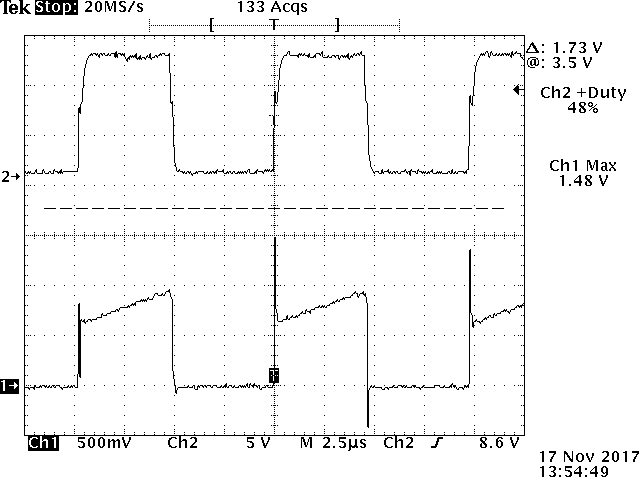
\includegraphics[max width=0.7\linewidth]{/tex/2iteration/billeder/Realisering/CS_U_filter.png}
	\caption{Oprindeligt current-sense signal før filter}
	\label{fig:CS_U_filter}
\end{figure}

\noindent Med den valgte stigetid på $100ns$, kan båndbredden af filteret estimeres:
\begin{equation} \label{filter_BW}
BW \approx \frac{0.34}{t_r} = \frac{0.34}{100ns} \approx 3.4M\hertz
\end{equation}

\noindent Kondensatoren fastholdes på $C_f=100pF$. Ud fra kondensatoren og den ønskede båndbredde i filteret, regnes modstanden.
\begin{equation} \label{filter_R}
R_f = \frac{1}{2 \cdot \pi \cdot BW \cdot C_f} = \frac{1}{2 \cdot \pi \cdot 3.4M\hertz \cdot 100pF} = 468.1\ohm
\end{equation}

\noindent Her vælges en modstand på $464\ohm$.






%%% Analyse for design af snubber-kredsløb til MOSFET og diode %%%

\section{Snubber-kredsløb}
Under 2. iteration blev det observeret under switching, blev der anslået svingninger på spændingen over både MOSFET'en og dioden. Disse højfrekvente svingninger vil, kunne støje på omkringliggende elektronik, både på printet og i rummet. Figur~\ref{fig:MOSFET_svingninger_2} og \ref{fig:diode_svingninger_2} viser problematikken i henholdsvis MOSFET og diode. Her er svingningerne i MOSFET'en tidligere blevet aflæst til at have en frekvens på $25M\hertz$, og svingningerne i dioden til at have en frekvens på $28.57M\hertz$. 

\begin{figure}[H]
	\center
	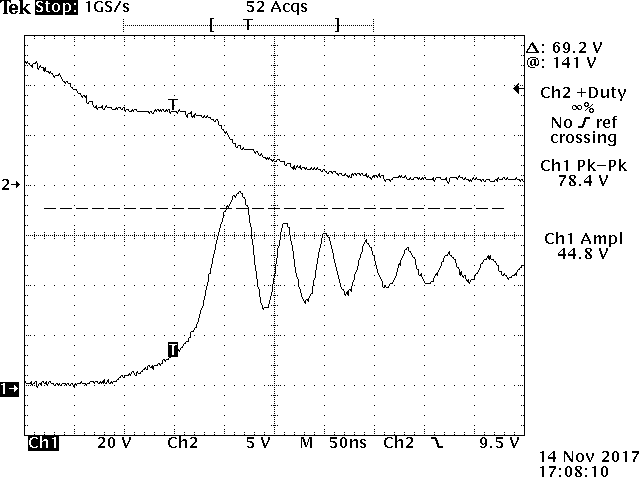
\includegraphics[max width=0.7\linewidth]{/tex/2iteration/billeder/Realisering/Transformator_Primarzoom.PNG}
	\caption{Svingninger i MOSFET}
	\label{fig:MOSFET_svingninger_2}
\end{figure}

\begin{figure}[H]
	\center
	\includegraphics[max width=0.7\linewidth]{/tex/2iteration/billeder/Realisering/Transformator_sekundarzoomrise.PNG}
	\caption{Svingninger i diode}
	\label{fig:diode_svingninger_2}
\end{figure}


Disse svingninger opstår som et biprodukt mellem spredningsselvinduktionen i transformatoren og kapaciteterne i henholdsvis MOSFET og diode. Den kapacitive kobling i transformatoren vil også have en påvirkning på frekvensen af svingningerne. De parasitiske komponenter er indtegnet på figur~\ref{fig:snubber_parasit}\cite{snubber_parasit}.  

\begin{figure}[H]
	\center
	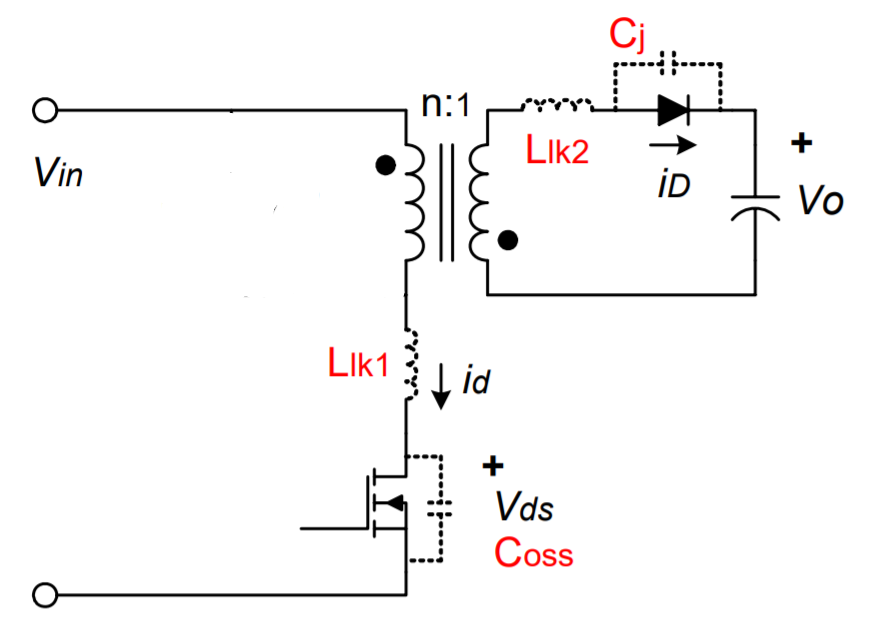
\includegraphics[max width=0.7\linewidth]{/tex/3iteration/billeder/Analyse/snubber_parasit.PNG}
	\caption{Parasitter i MOSFET, diode og transformator}
	\label{fig:snubber_parasit}
\end{figure}

Princippet i et snubber-kredsløb er, at udligne svingningerne med en kondensator, samt bruge en modstand til, at afsætte effekten fra svingningerne i. Derfor vil en konsekvens af, at bruge snubber-kredsløb være et større tab. Det er dog et nødvendigt tab for ikke at generere højfrekvent støj. 

Der er generelt to forskellige snubber-kredsløb der bliver brugt til, at fjerne disse svingninger - en RC-snubber og en RCD-snubber\cite{snubber_design}. En RC-snubber er en modstand og en kondensator i serie. Den bliver primært brugt til at fjerne svingningerne over dioden, men kan også bruges på MOSFET'en. Denne form for snubber er simpel at designe når man kender spredningsselvinduktionen i transformatoren, og er tilstrækkelig til at fjerne svingningerne. En RCD-snubber er en diode placeret i serie med en parallelforbindelse mellem en kondensator og en modstand. Den bruges ofte kun på primærsiden og er placeret over transformatorviklingen. Denne form for snubber er mere kompliceret at designe, og kræver flere komponenter. Derfor vælges det at bruge RC-snubbere på både primær- og sekundærsiden.

Det startes med, at designe kredsløbet til MOSFET'en. Her blev svingningerne aflæst til en frekvens på $25M\hertz$. Ved at bruge spredningsselvinduktionen i transformatoren og svingningsfrekvensen, kan den resulterende kapacitet regnes ved, at løse følgende ligning.
\begin{equation} \label{eq:MOSFET_snubber}
f = \frac{1}{2 \cdot \pi \cdot \sqrt{L_{m} \cdot C_{pri}}} \Rightarrow C_{pri}=266.6pF
\end{equation}

Kondensatoren i snubber kredsløbet bør være ca. $2-3$ gange større end den beregnede kapacitet\cite{snubber_design}. Der vælges en faktor 2:
\begin{equation}
C_{snubM} = 2 \cdot C_{pri} = 533.6pF
\end{equation}

\noindent Det vælges at runde op til $600pF$, da denne værdi kan realiseres. For optimal dæmpning bør impedansen af modstanden, være lig impedansen i spredningsselvinduktionen, ved svingningsfrekvensen. 
\begin{equation}
R_{snubM} = 2 \cdot \pi \cdot L_m \cdot f = 2 \cdot \pi \cdot 152nH \cdot 25M\hertz = 23.9\ohm
\end{equation}

\noindent Her rundes ned til $23.7\ohm$ da denne kan realiseres. 

\noindent For design af snubber-kredsløbet til dioden bruges samme fremgangsmåde.
\begin{equation} \label{eq:diode_snubber}
f = \frac{1}{2 \cdot \pi \cdot \sqrt{L_{m} \cdot C_{sek}}} \Rightarrow C_{sek}=204.1pF
\end{equation}

Igen vælges det, at gøre $C_{snubD}$ en faktor 2 større end $C_{sek}$:
\begin{equation}
C_{snubD} = 2 \cdot C_{sek} = 408.2pF
\end{equation}

\noindent Det vælges at runde ned til $400pF$, da denne værdi kan realiseres. Modstanden dimensioneres ud fra impedansen i spredningsslevinduktionen. 
\begin{equation}
R_{snubD} = 2 \cdot \pi \cdot L_m \cdot f = 2 \cdot \pi \cdot 152nH \cdot 28.6M\hertz = 27.3\ohm
\end{equation}

\noindent Her rundes op til $27.4\ohm$ da denne kan realiseres.




%%% Analyse af optimering af udgangsfilter %%%

\section{Udgangsfilter}
I 2. itertion blev udgangsfilteret realiseret ved fire $56\micro F$ film kondensatorer i parallel. Filteret er vist på figur~\ref{fig:udgangsfilter_2} hvor selve filteret er de fire blå kondensatorer, og udgangen er bananstikkene placeret til venstre. 


\begin{figure}[H]
	\center
	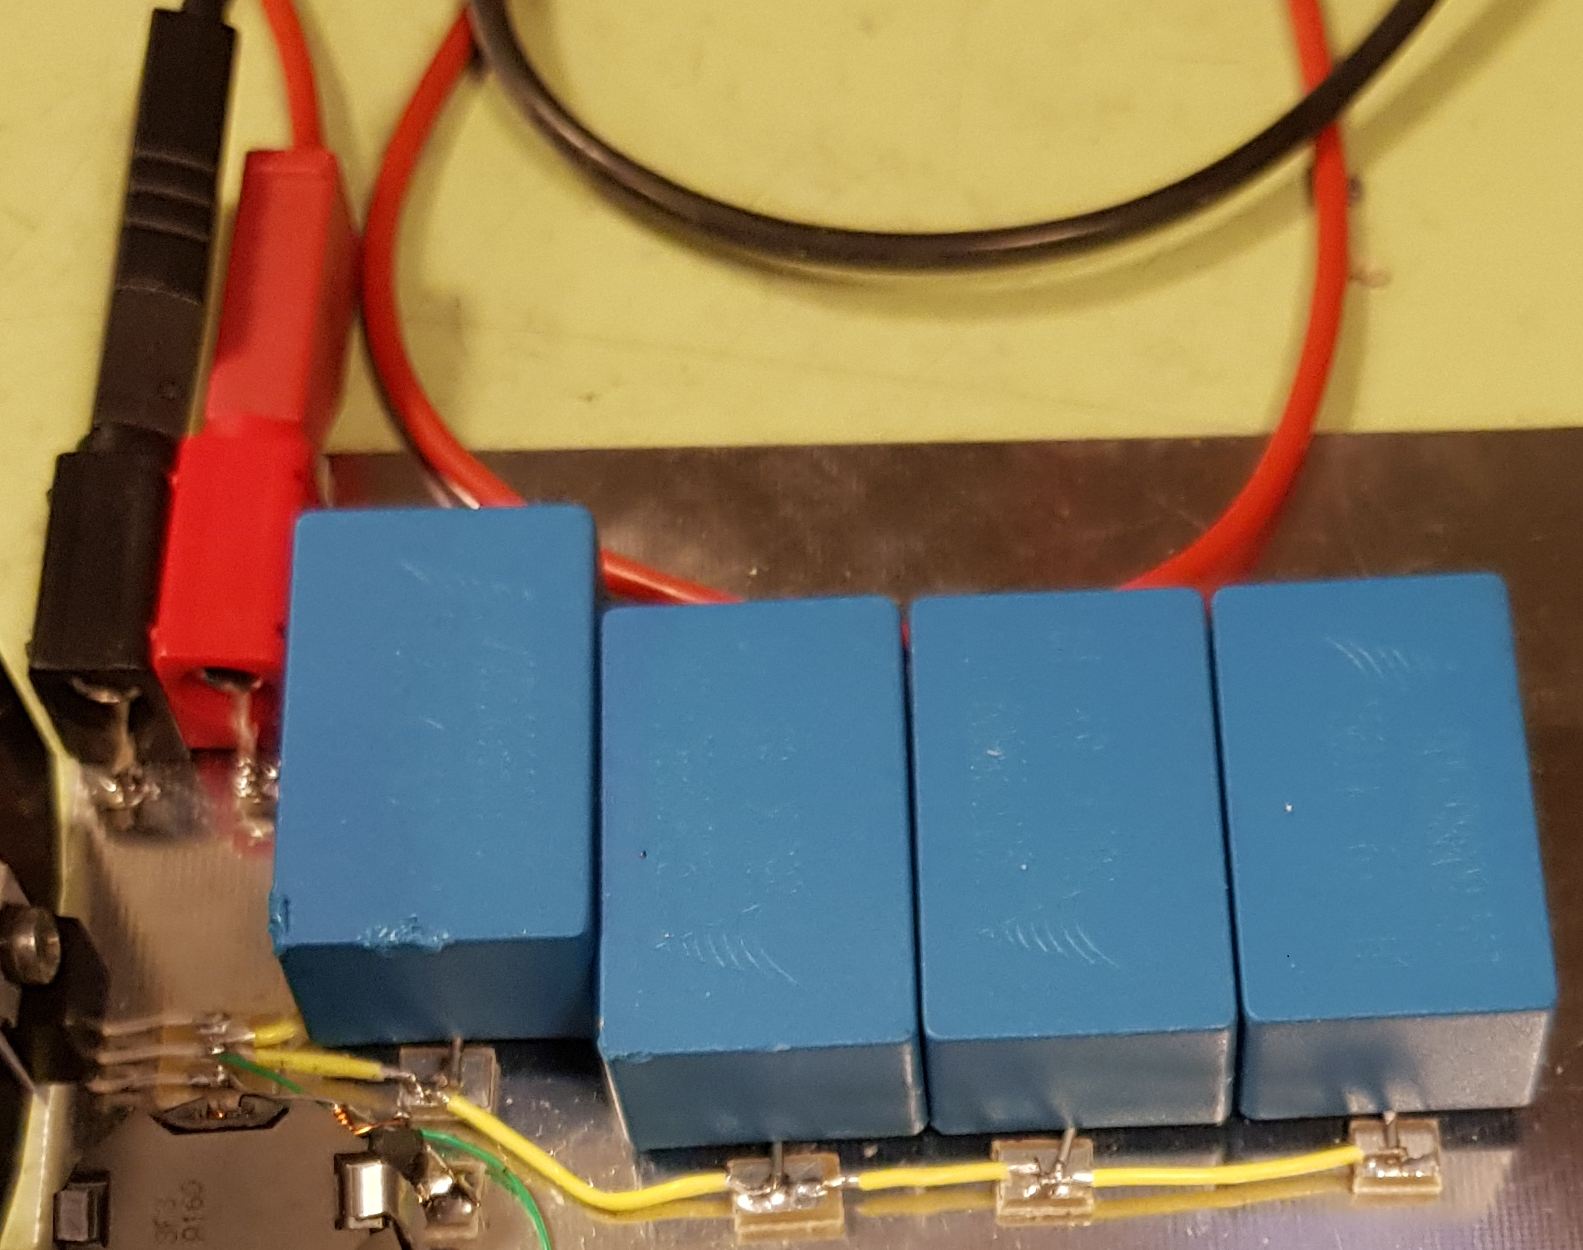
\includegraphics[max width=0.7\linewidth]{/tex/3iteration/billeder/Analyse/Udgangsfilter_2iteration.png}
	\caption{Implementeret udgangsfilter - 2. iteration}
	\label{fig:udgangsfilter_2}
\end{figure}

Denne implementering af udgangsfilteret, medførte switchin-spikes på udgangen op mod $5V pk-pk$. Dette er vist på figur~\ref{fig:output_2}, hvor kanal 1 viser udgangen, og kanal 2 viser MOSFET'ens gate. Disse spikes ønskes mindsket. I afsnit~\ref{output_cap} blev det beskrevet, at det som hovedregel kan antages, at en ledning har en selvinduktion på $1nH/mm$. Bruges den antagelse på udgangsfilteret, kan ledningerne mellem kondensaterne moduleres som spoler. Det betyder, at hver kondensator er en del af et LC-filter, som hver især filtrere højfrekvente signaler på udgangen. 


\begin{figure}[H]
	\center
	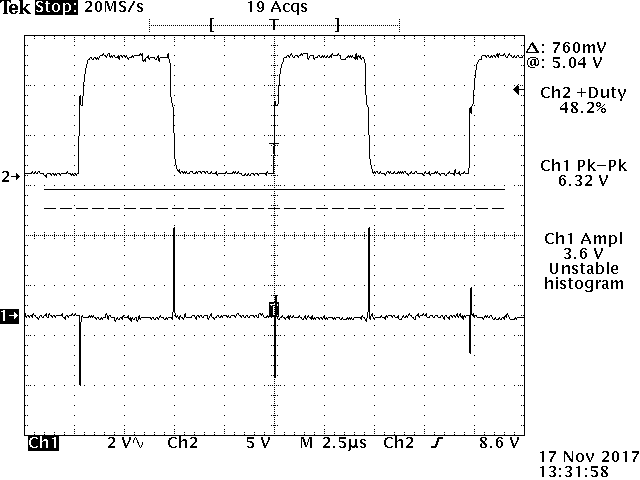
\includegraphics[max width=0.7\linewidth]{/tex/2iteration/billeder/Realisering/Output_26V.png}
	\caption{Output - 2. iteration}
	\label{fig:output_2}
\end{figure}

Det antages at hver ledning i gennemsnit er ca. $30mm$, hvilket giver en selvinduktion på ca. $30nH$. Der regnes en knækfrekvens for filteret ved ligning~\ref{out_filter}. Det viser, at knækfrekvensen for filtret ligger tæt på den brugte switch-frekvens, hvilket ikke er optimalt. Det vurderes dog, at den ligger højt nok, til ikke at have en påvirkning på det egentlige udgangssignal. Tilsammen vil de fire kondensatorer dermed virke som et 8. ordensfilter med en knækfrekvens på ca. $122.8k\hertz$. Ud fra den analyse vælges det, at flytte udgangen til den anden ende af udgangsfilteret, for dermed at udnytte denne filtrering. 

\begin{equation} \label{out_filter}
f = \frac{1}{2 \cdot \pi \cdot \sqrt{C_{out} \cdot L_{out}}} = \frac{1}{2 \cdot \pi \cdot \sqrt{56\micro F \cdot 30nH}} = 122.8k\hertz
\end{equation}

I kombination med kondensatorens resonans frekvens på $108k\hertz$, regnet i afsnit~\ref{output_cap}, burde der findes en ny kondensator i en senere iteration. 



%%% Analyse for optimering af reguleringsloop %%%


\section{Gain-fase}
Reguleringssløjfen optimeres for, at opnå en større båndbredde. En større båndbredde vil give en hurtigere respons i systemet. Det vil betyde at systemet hurtige begynder at regulere ind ved ændringer på indgangen eller på loaden. Det resulterer i, at overshootet vil blive mindre.  

Der tages udgangspunkt i bode plottet for power modulet på figur~\ref{fig:MATLAB_power_module}. Ud fra kravene der er opstillet i afsnit~\ref{krav}, skal systemet minimum have en gain-margin på $10\decibel$ og en fase-margin på $50^\circ$. Ud fra figur~\ref{fig:MATLAB_power_module} ses det, at hvis der skal opnås en gain-margin på $10\decibel$, skal der tilføres en forstærkning på $8.5\decibel$. Ud fra bode plottet aflæses det, at ved, at løfte forstærkningen med $8.5\decibel$, vil der opnås en fase-margin på ca. $75^\circ$ og en båndbredde på ca. $4k\hertz$. 

\begin{figure}[H]
	\center
	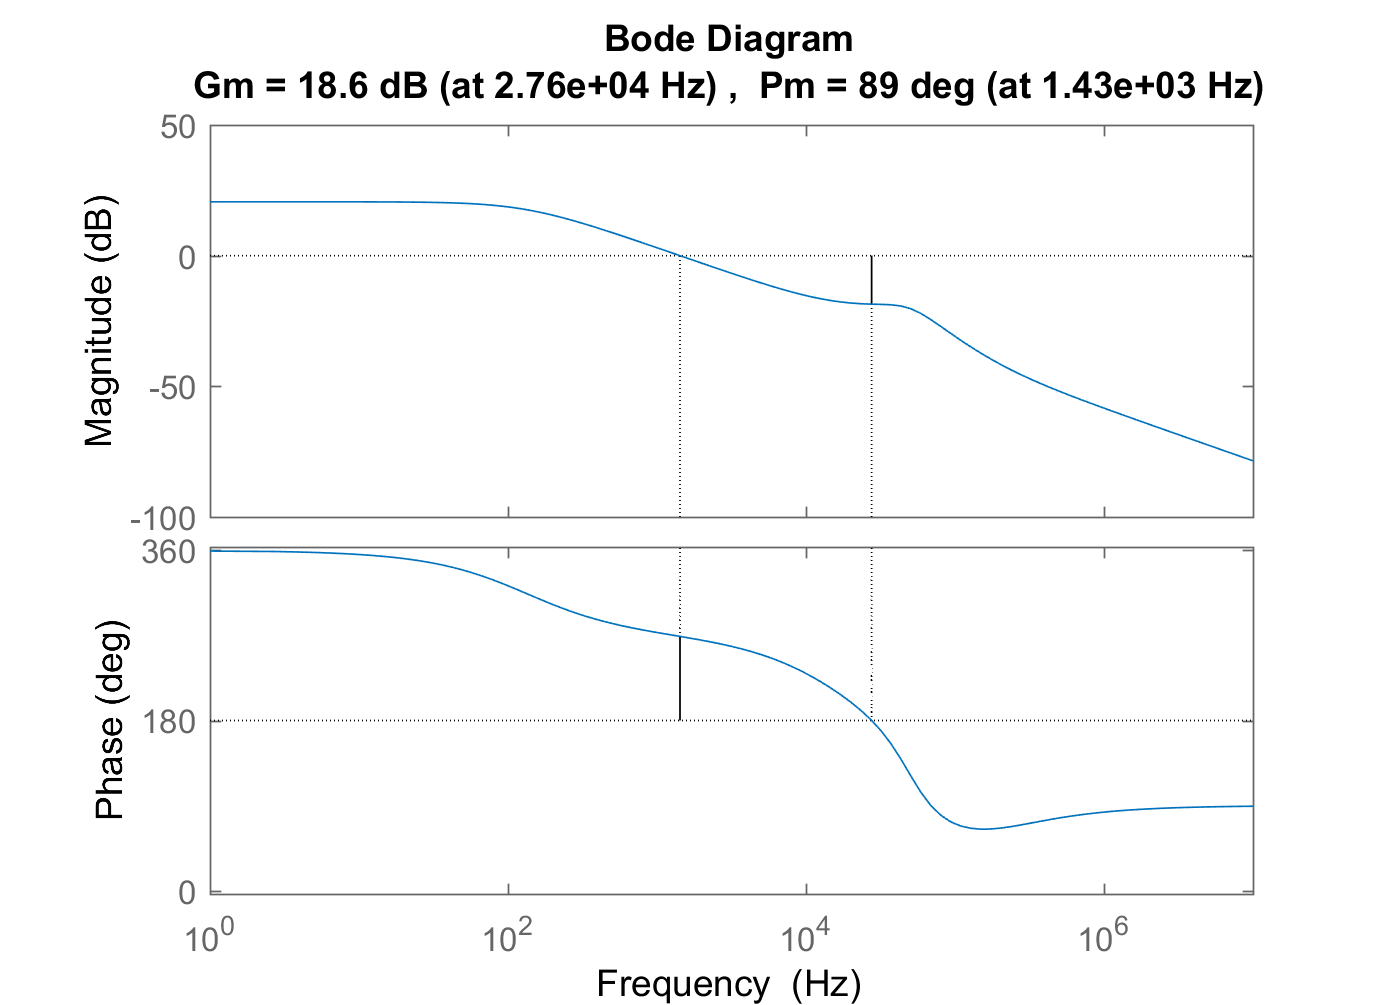
\includegraphics[max width=0.7\linewidth]{/tex/2iteration/billeder/MATLAB_power_module.PNG}
	\caption{Bode plot for power-modulet}
	\label{fig:MATLAB_power_module}
\end{figure}

\noindent Fremgangsmåden er den samme som ved 2. iteration. Feedback modstanden i fejlforstærkeren regnes ved at løse ligning~\ref{error_opamp_gain_3}.

\begin{equation} \label{error_opamp_gain_3}
g_{tot} = \frac{R_{comp}}{R_{par}} \cdot g_{FB}
\end{equation}

\noindent Hvor:
\newline \noindent $g_{tot}$ er den ønskede forstærkning i fejlforstærkeren. Der ønskes en forstærkning på $g_{totdb}8.5\decibel \Rightarrow g_{tot}=2.66gg$.
\newline \noindent $R_{comp}$ er feedbackmodstanden i fejlforstærkeren, som ønskes dimensioneret.
\newline \noindent $R_{par}$ er parallelmodstanden mellem $R_{FB1}$ og $R_{FB2}$. Den regnes til $R_{par}=2.244k\ohm$.
\newline \noindent $G_{FB}$ er forstærkningen i spændingsdeleren, og er tidligere regnet til $G_{FB}=0.12GG$.

\noindent De kendte værdier indsættes og ligningen løses for $R_{comp}$. Den fås til $R_{comp} = 49.8k\ohm$. Her rundes op til $49.9k\ohm$, som kan skaffes.

På figur~\ref{fig:MATLAB_total_2}, som er bodeplottet for det samlede system ved 2. iteration, ses det at fasen får et dyk, mellem ca. $80\hertz$ og ca. $400\hertz$. Det kommer fordi polen ved $132\hertz$ trækker fasen ned, mens det nulpunkt der er indsat ved $318\hertz$ trækker fasen op. Ved at flytte de punkter til samme frekvens, opnås en konstant fase ved lavere frekvenser. Derfor flyttes frekvensen for nulpunktet til $f_0=132\hertz$. Ud fra den nye modstand, og den nye knækfrekvens, regnes den nye kondensator. Det afrundes til $24.2nF$, da det kan skaffes.
\begin{equation} \label{c_comp_3}
c_{comp} = \frac{1}{2\cdot \pi \cdot R_{comp} \cdot f_0} = 24.1nF
\end{equation}

\noindent Det giver en ny overføringsfunktion for fejlforstærkeren, der skrives ved ligning~\ref{G_err_3}. 
\begin{equation} \label{G_err_3}
G_{err}(s) = (\frac{132.8\hertz \cdot 2\cdot\pi}{s} + 1) \cdot 2.66
\end{equation}

\noindent Den plottes i MATLAB, som et bodeplot på figur~\ref{fig:MATLAB_error_op_amp_3}. Her ses det, at den ønskede funktion af fejlforstærkeren er opnået, da forstærkningen ved frekvenser over $132\hertz$ er $8.54\decibel$. 

\begin{figure}[H]
	\center
	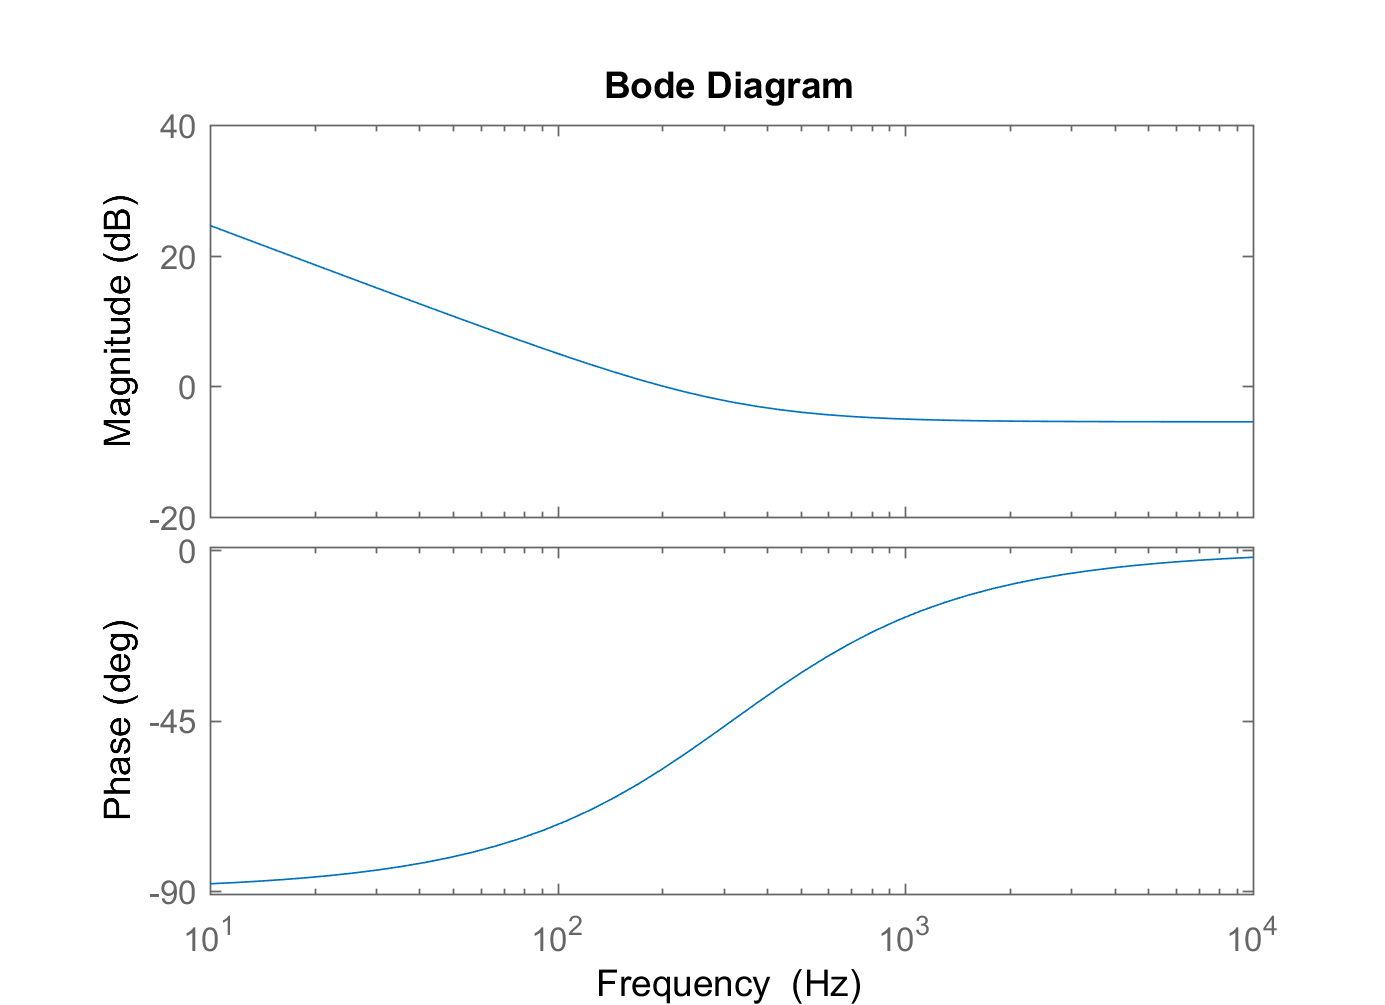
\includegraphics[max width=0.7\linewidth]{/tex/3iteration/billeder/Analyse/MATLAB_error_op_amp.PNG}
	\caption{Bode plot for fejlforstærker}
	\label{fig:MATLAB_error_op_amp_3}
\end{figure}

\noindent Den nye overføringsfunktion for fejlforstærkeren, ganges sammen med overføringsfunktionen for power modulet. Figur~\ref{fig:MATLAB_total_3} viser et bode plot af det samlede system. Det aflæses at converteren vil få en gain-margin på de forventede $10\decibel$, en fasemargin på $72.7^\circ$, og en båndbredde på ca. $3.94k\hertz$. Derudover kan det konstateres at nulpunktet er blevet placeret efter hensigten, da fasen ligger forholdsvis konstant ved frekvenser under $1k\hertz$. 

\begin{figure}[H]
	\center
	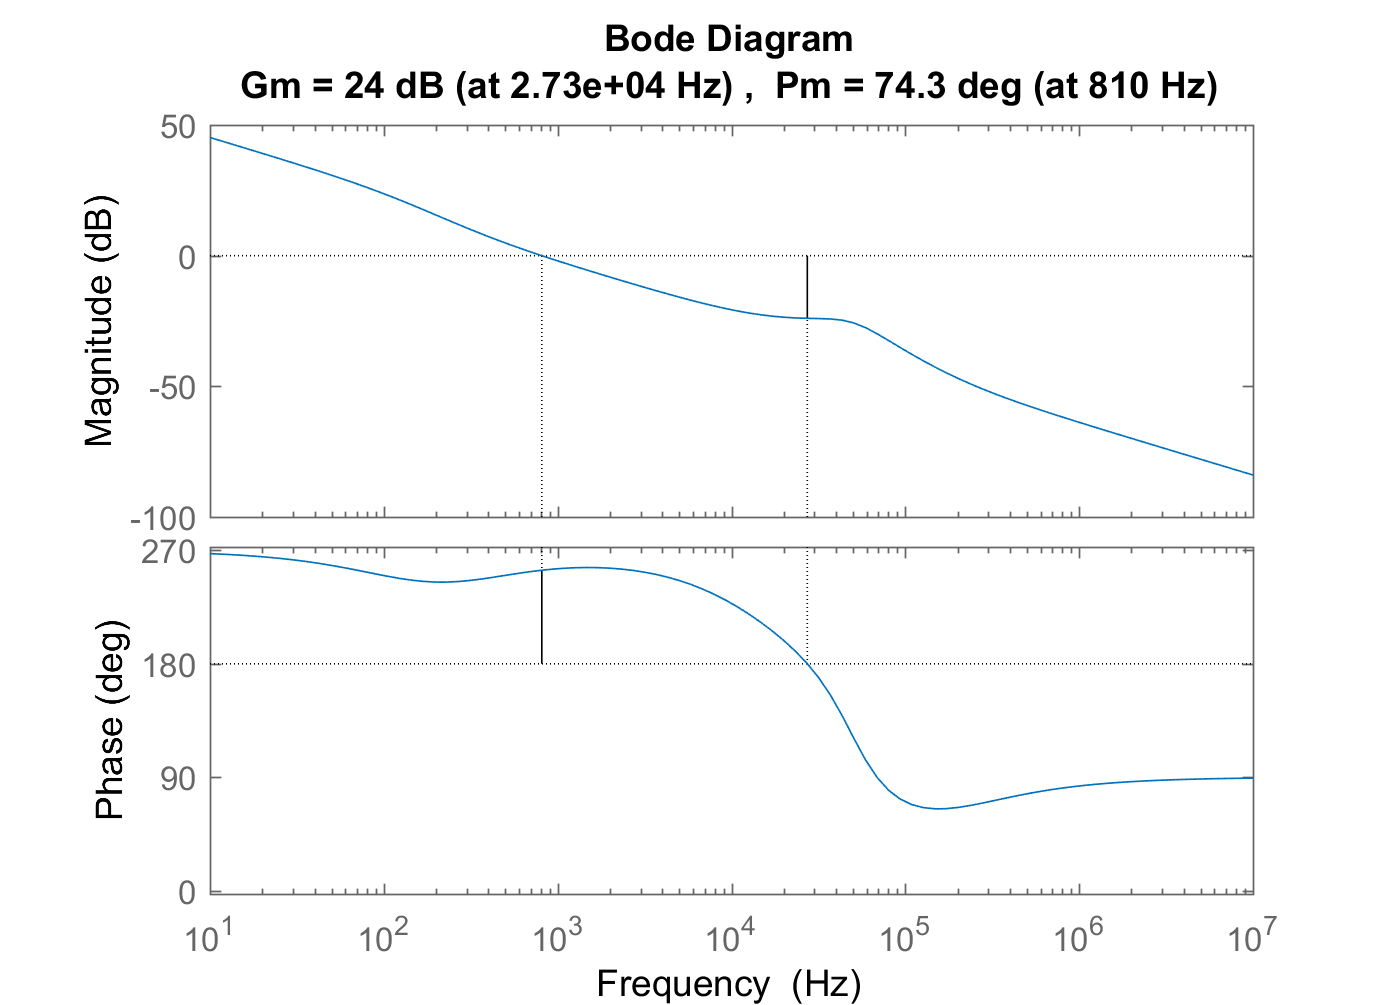
\includegraphics[max width=0.7\linewidth]{/tex/3iteration/billeder/Analyse/MATLAB_total.PNG}
	\caption{Bode plot for det samlede system}
	\label{fig:MATLAB_total_3}
\end{figure}








\subsection{Tab}
Som konsekvens af nogle af optimeringerne, har tabet ændret sig i systemet. I denne sektion gennemgås de steder hvor tabet har ændret sig og slutter af med de nye samlede tab i konverteren.

\subsubsection{MOSFET}
Switchtabet i MOSFET'en er ændret idet gate-modstanden er gjort mindre. Det har givet en fornyet switch tid på 37.2ns. Dette tab udregnes på samme måde som i sektion ~\ref{switchtab2}. Med ligningen derfra fås et fornyet switch tab på:
\begin{equation}
P_{switch} = \frac{1}{2} \cdot I_{pkavg21} \cdot (V_{inmax}+V_{out21}) \cdot \frac{(t_r+t_f)}{T}= 1.48\watt
\end{equation} 
Der er altså et switchtab på $3\watt$ mindre efter switchtiden er blevet ændret. 
Det ændrer det samlede tab i MOSFET'en til $2.54\watt$

\subsubsection{Snubber-kredsløb}
Ulempen ved at indsætte snubber-kredsløbene er det ekstra tab der kommer i modstandene. Tabet i modstanden findes ved at tage kapaciteten i kondensatoren ganget med spændingen over modstanden i anden og switchfrekvensen.
Det giver følgdende snubber tab ved MOSFET og diode.
\begin{equation}
P_{snubM} = C_{snubM}\cdot {80V}^{2}*f_s = 0.341\watt
\end{equation} 

\begin{equation}
P_{snubD} = C_{snubM}\cdot {70V}^{2}*f_s = 0.2\watt
\end{equation}
\fxnote{Udledning af formel? Spænding over kondensator udregning?}
 

\clearpage

\section{Simulering}
I dette afsnit laves simuleringer for optimerede, og nye kredsløb for 3. iteration. Her der er to større ændring ift. 2. iteration - indsat snubber-kredsløb på både primær- og sekundærsiden, samt en mere præcis modulering af udgangsfilteret. Derudover er der ændret komponentværdier ifm. optimering af allerede udviklede kredsløb. Disse ændringer vil blive beskrevet nærmere med diagram tegninger i de relevante afsnit. 

%%% Simulering for optimering af gate-modstand %%%

\subsection{Switch-tid}
Den optimerede switch-tid simuleres ved at måle spændingen på MOSFET'ens gate. Det signal er vist på figur~\ref{fig:switch_tid_3}. Her aflæses switch-tiden til ca. $29ns$. Denne værdi afviger af samme grund som ved 2. iteration. Da der jo er brugt en anden model i p-spice ende den tiltænkte, passer \textit{Miller} ladningen ikke. Ved 2. iteration blev den aflæst til ca. $15nC$, og regnes den switch-tiden ved denne ladning bliver det:
\begin{equation} 
T_{ch} = \frac{Q_{gd} \cdot R_{g}}{V_{DD}-V_{gs}} = \frac{15nC \cdot 13.7\ohm}{12V-5V} = 29.4ns
\end{equation}

\begin{figure}[H]
	\center
	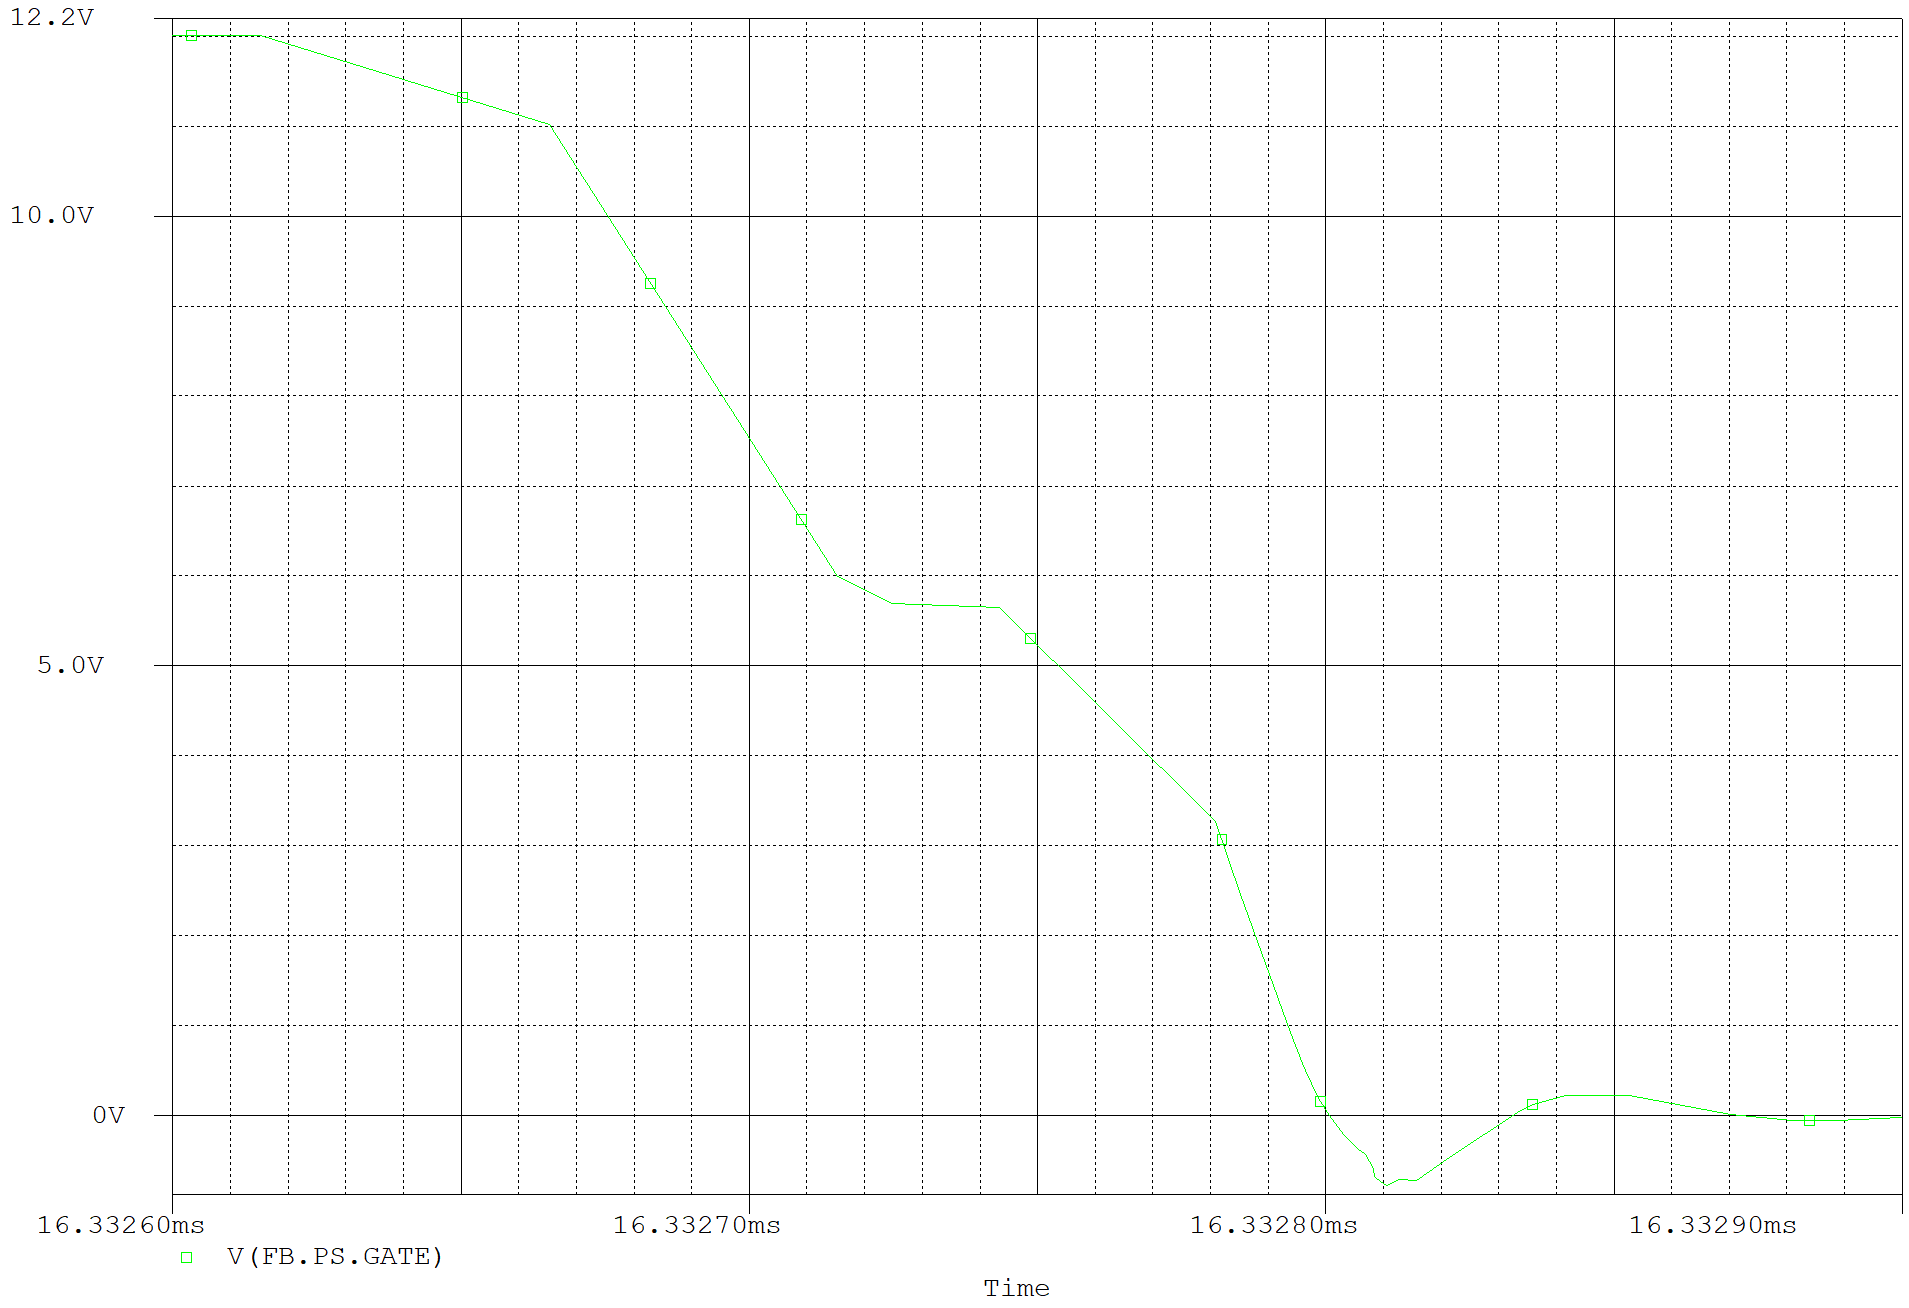
\includegraphics[max width=0.7\linewidth]{/tex/3iteration/billeder/Simulering/Simulering_switch_tid.png}
	\caption{Switch-tid for MOSFET - 3. iteration}
	\label{fig:switch_tid_3}
\end{figure}

En af konsekvenserne ved en hurtigere switch-tid er, som nævnt i afsnit~\ref{sec:switch_tid}, at peak'en på spændingen over MOSFET'ens drain bliver større. Dette er målt ved figur~\ref{fig:switch_tid_peak}. spændingen aflæses til at have en peak på $110V$. Det er en margin på $27\percent$ til MOSFET'ens breakdown spænding, hvilket godtages. 

\begin{figure}[H]
	\center
	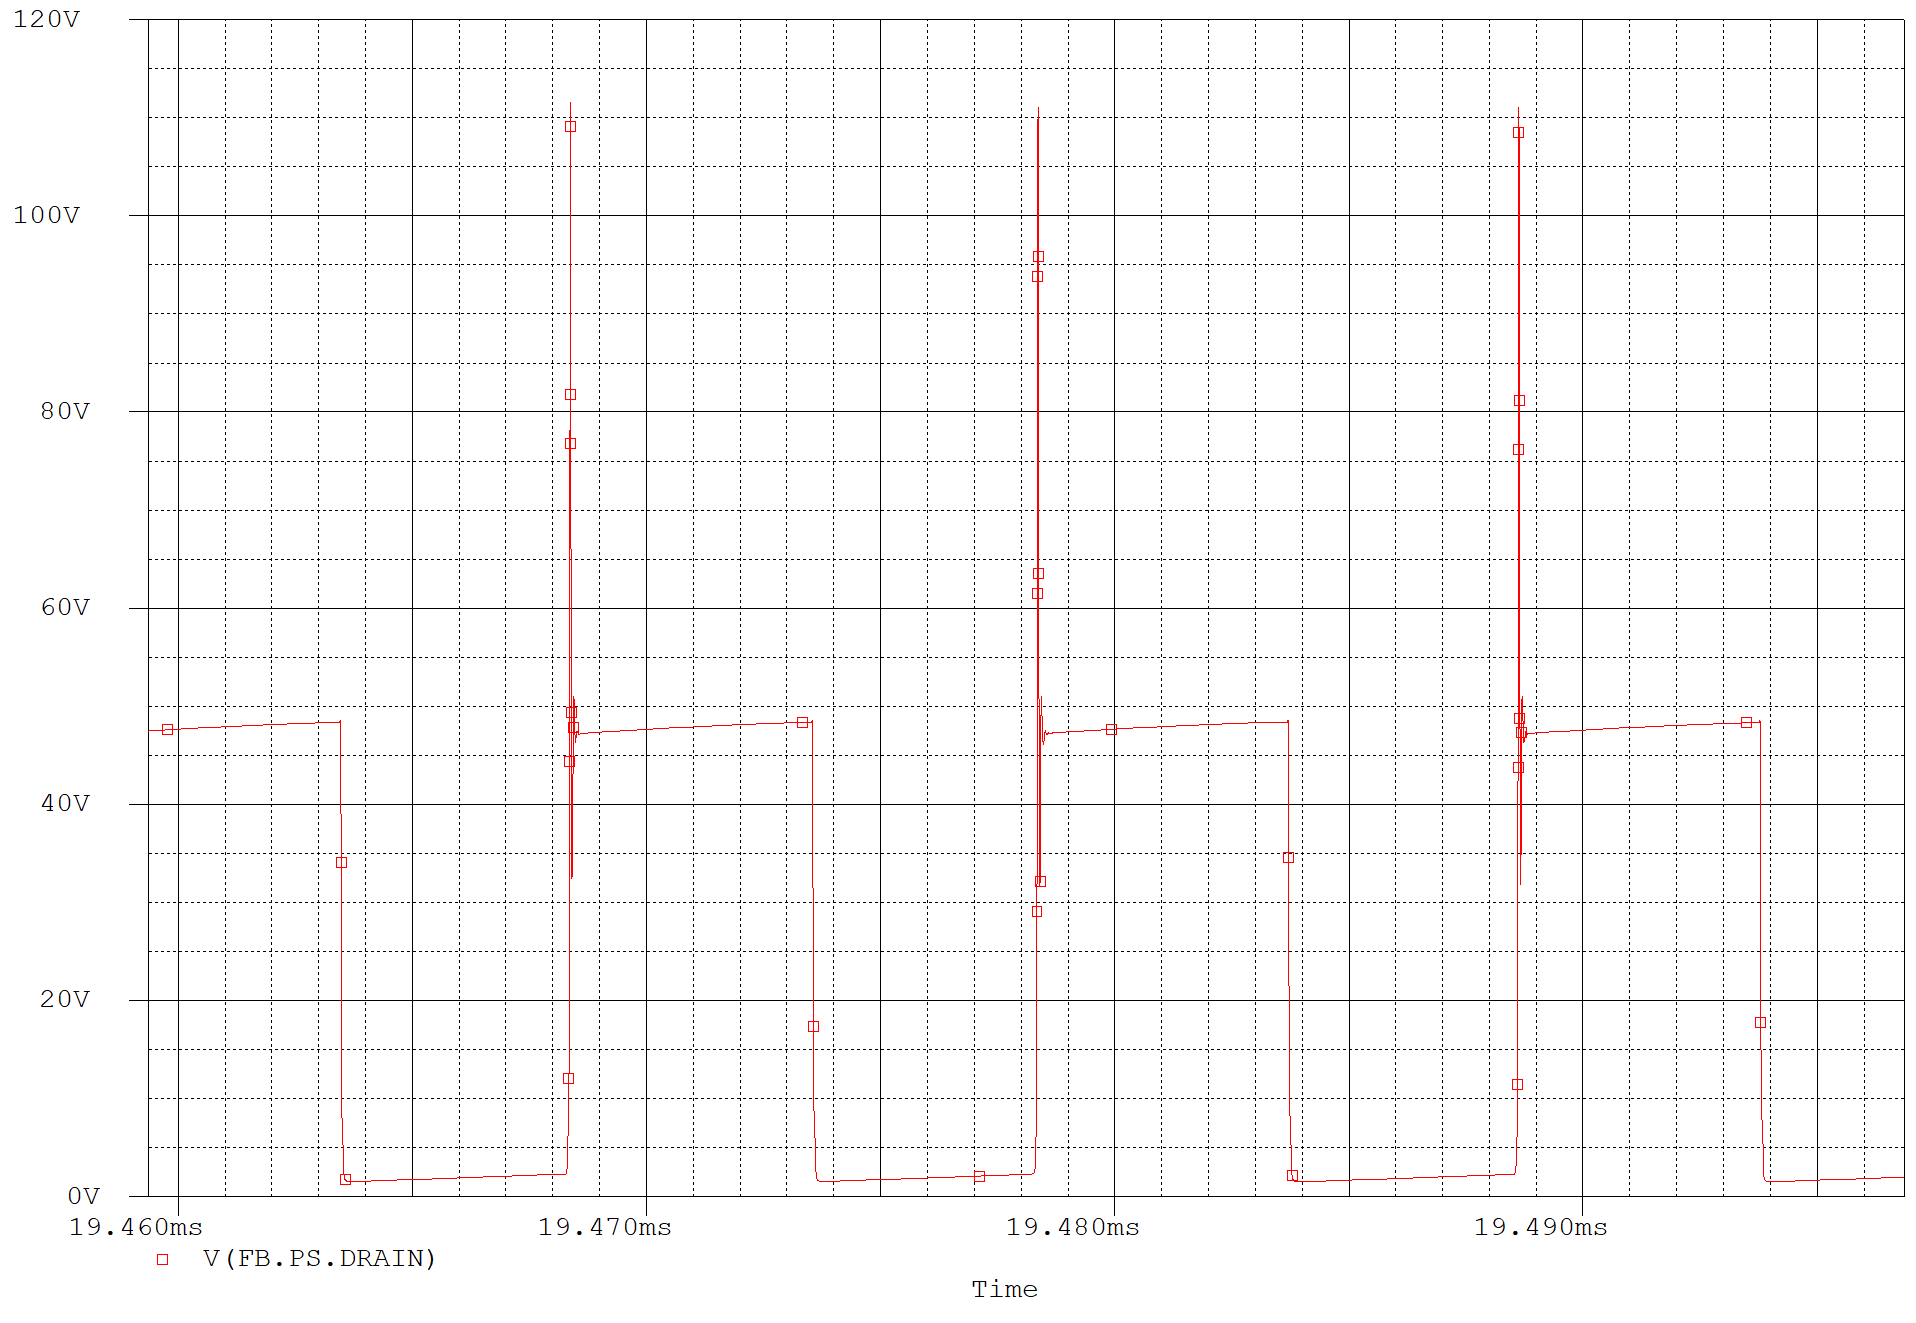
\includegraphics[max width=0.7\linewidth]{/tex/3iteration/billeder/Simulering/Simulering_switch_tid_peak.png}
	\caption{MOSFET drain - 3. iteration}
	\label{fig:switch_tid_peak}
\end{figure}

%%% Simulering for optimering af Current-sense filter %%%

\subsection{Current-sense filter}
Simuleringen af current-sense filteret sker ved, at måle current-sense signalet både før og efter filteret. Figur~\ref{fig:Simulering_PWM_current_sense_U_3} viser det ufiltrerede signal. Her ses stadig de forventede switching-spikes. Figur~\ref{fig:Simulering_PWM_current_sense_M_3} viser det filtrerede signal. Her aflæses stigetiden til ca. $85ns$, og derfor en hurtigere stigetid end det analyserede. Den hurtigere stigetid godtages, da switching-spikes'ene stadig er blevet filtreret væk. Det ses dog, at der kommer et lille overshoot på signalet. Det betyder at filterets stigetid kun lige præcis er lang nok til, at filtrer spikes'ene. 

\begin{figure}[H]
	\center
	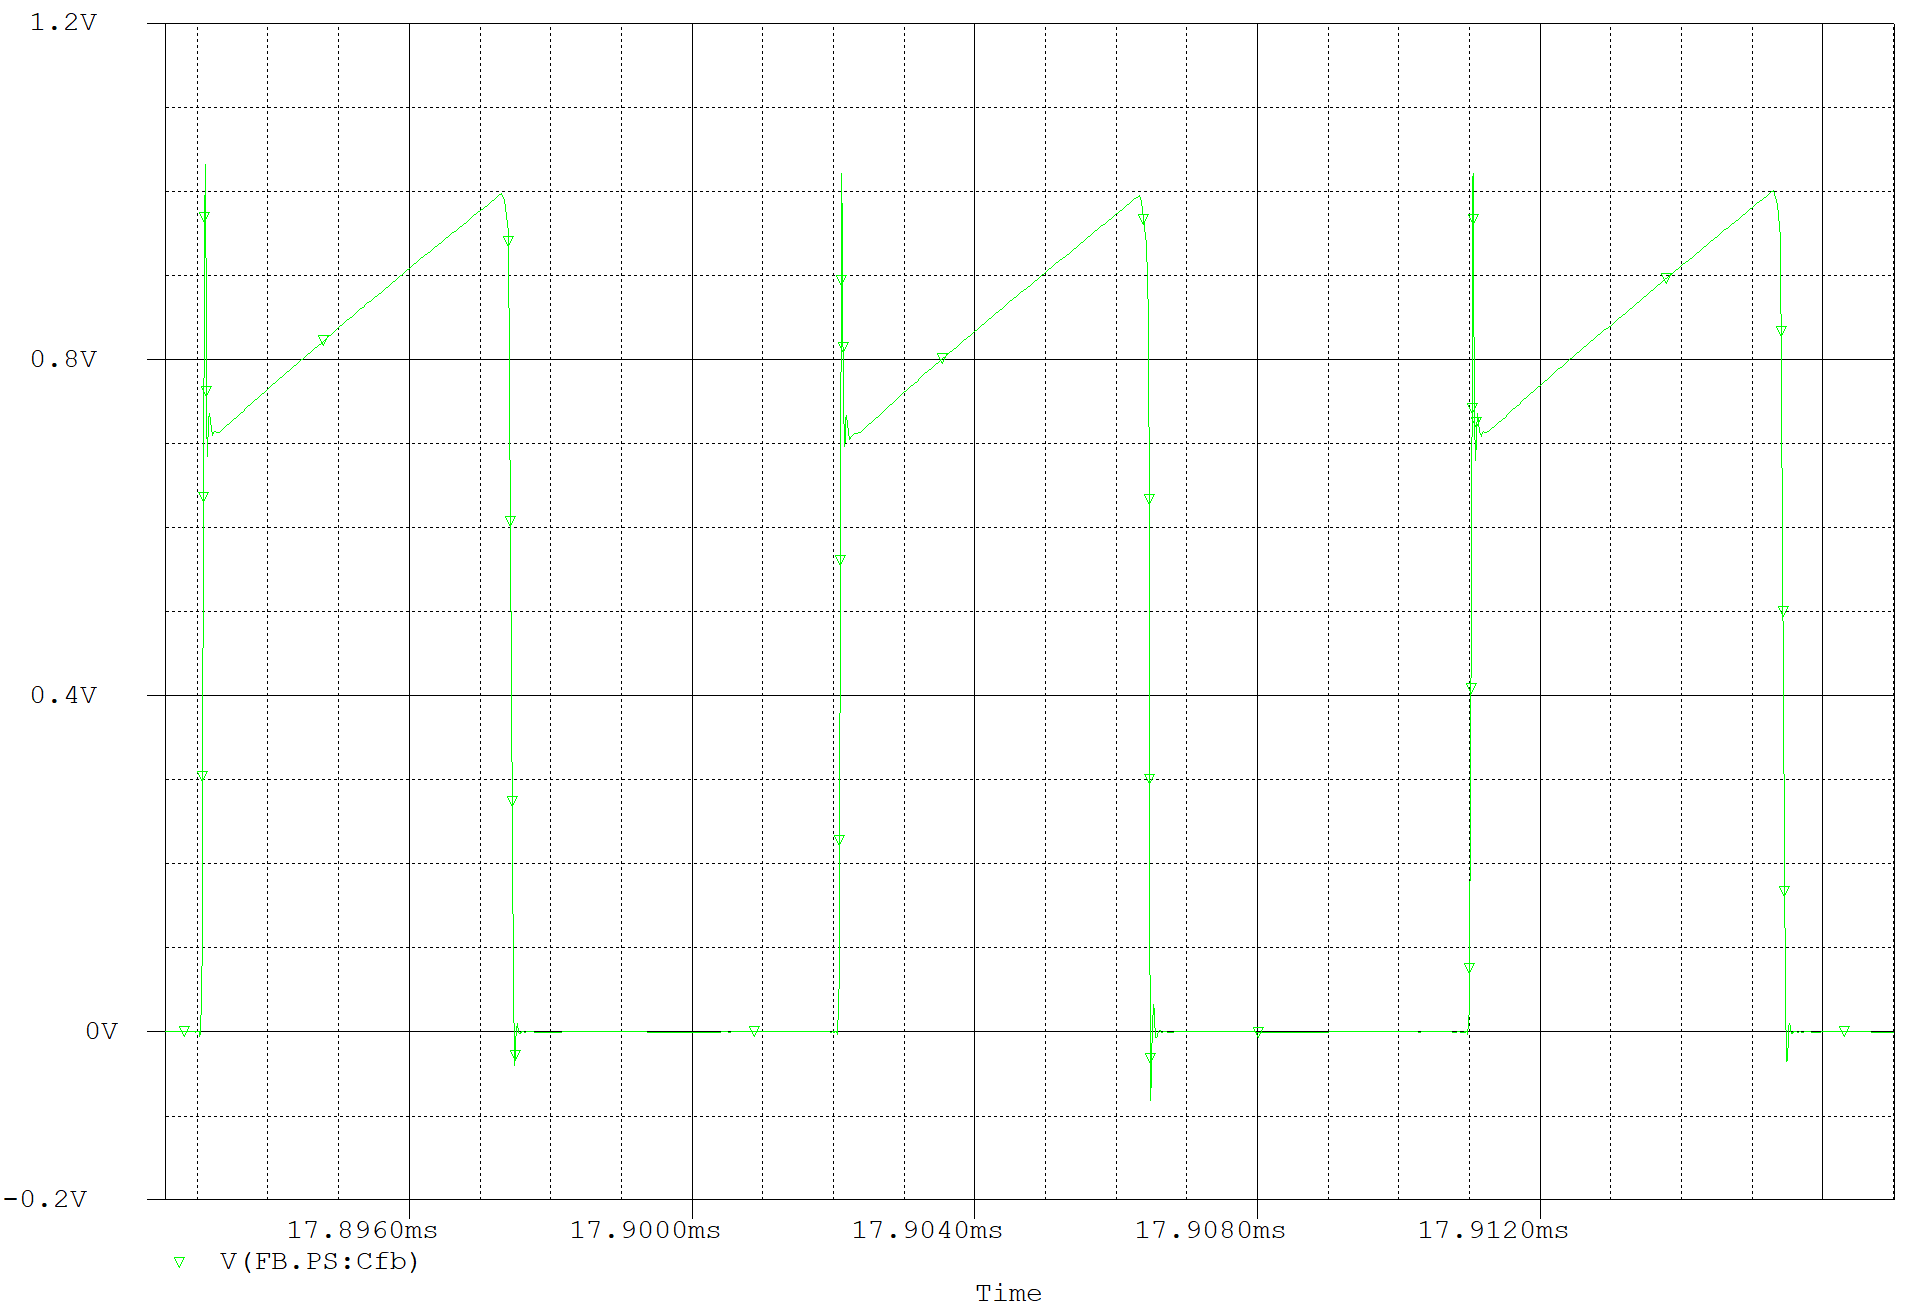
\includegraphics[max width=0.7\linewidth]{/tex/3iteration/billeder/Simulering/Simulering_cs_filter_U.png}
	\caption{Simulering af current-sense signal før filtrering}
	\label{fig:Simulering_PWM_current_sense_U_3}
\end{figure}

\begin{figure}[H]
	\center
	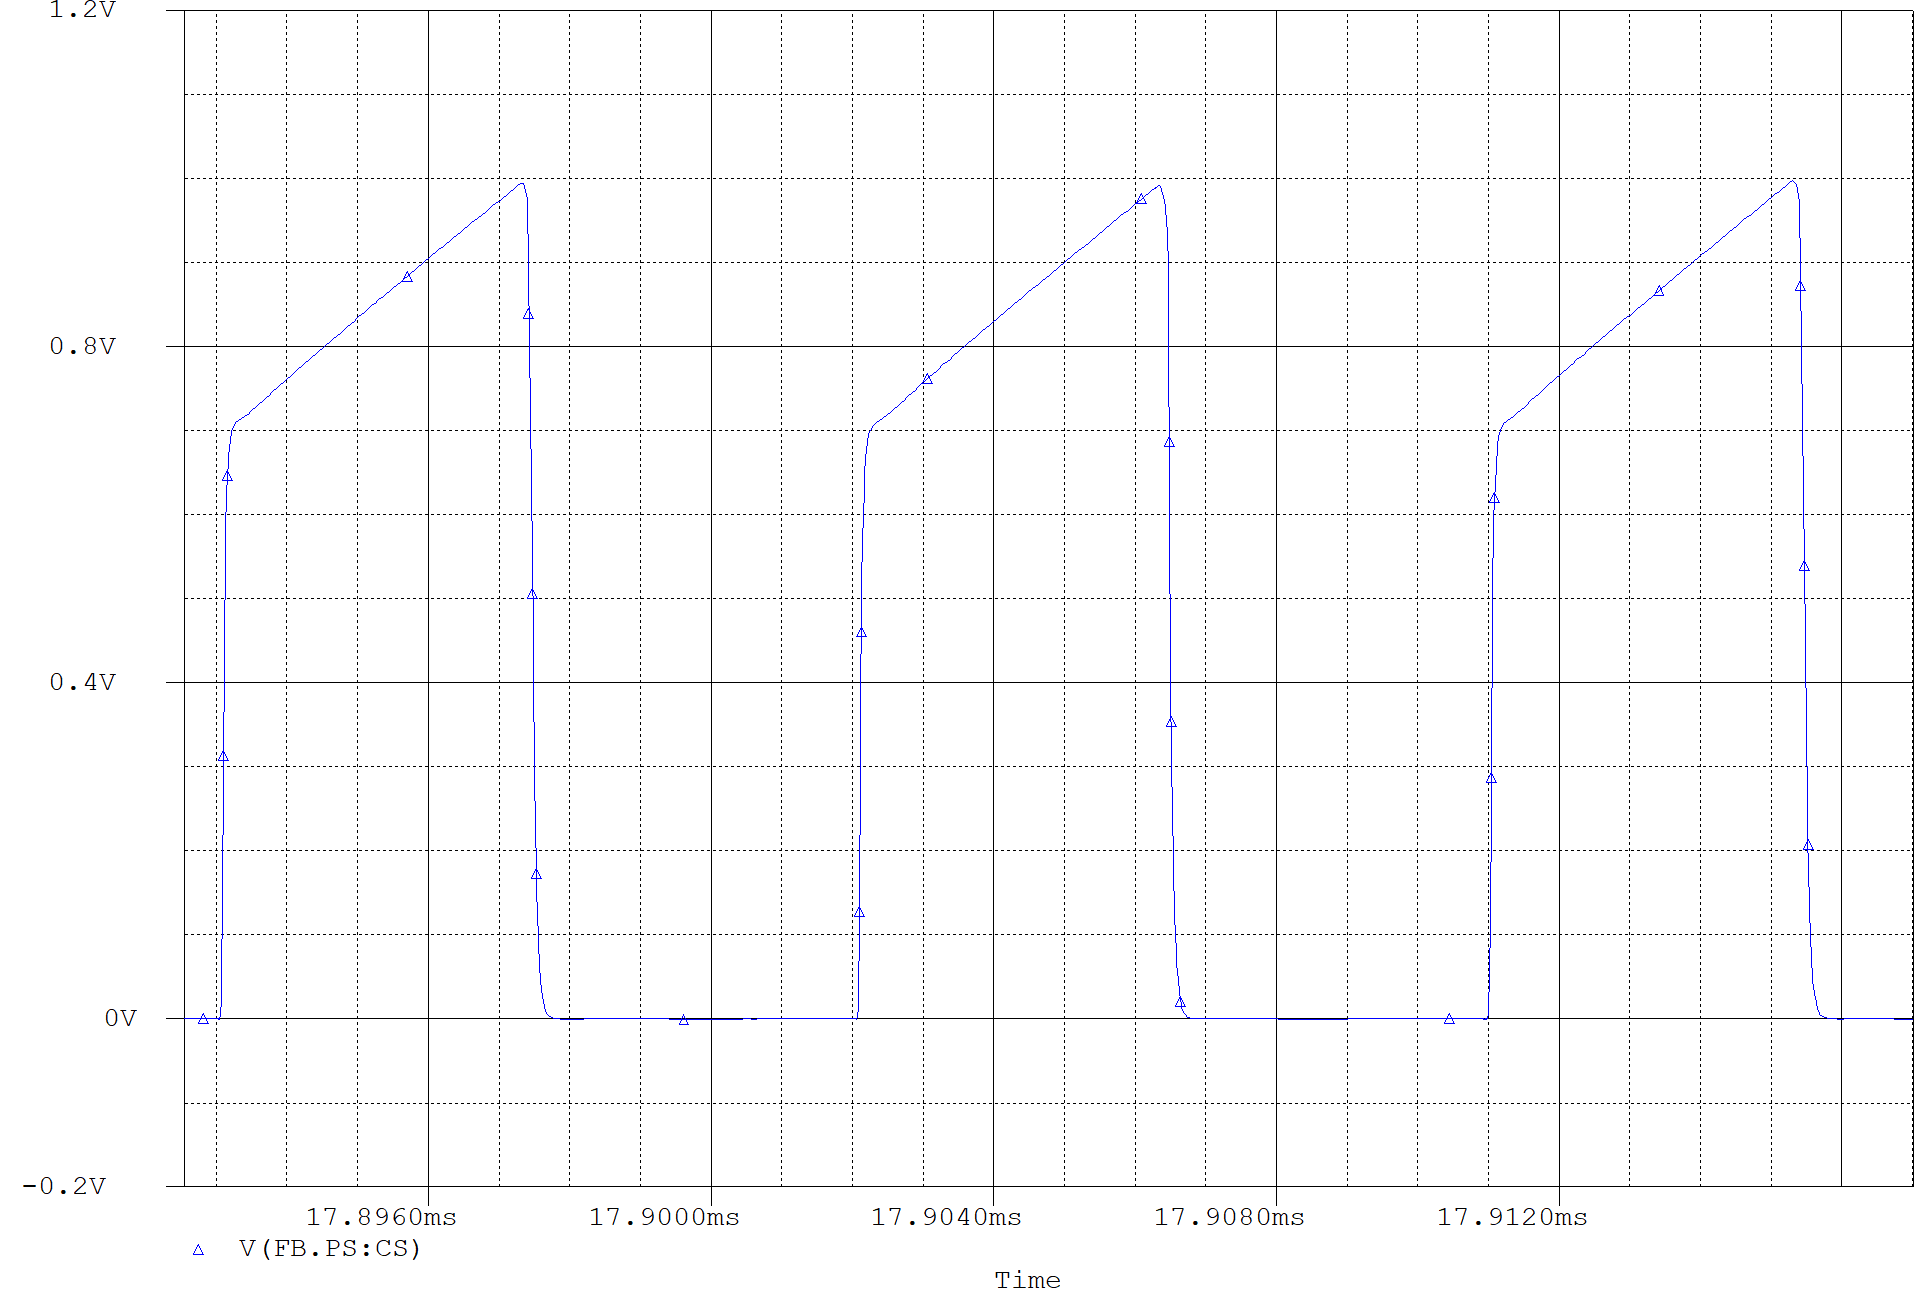
\includegraphics[max width=0.7\linewidth]{/tex/3iteration/billeder/Simulering/Simulering_cs_filter_M.png}
	\caption{Simulering af current-sense signal efter filtrering}
	\label{fig:Simulering_PWM_current_sense_M_3}
\end{figure}

%%% Simulering for design af snubber-kredsløb til MOSFET og diode %%%

\subsection{Snubber-kredsløb}
Figur~\ref{fig:simulering_diagram_snubber_3} viser det opdaterede diagram med snubber-kredsløbene indsat. Her ses det at primær-snubberen er placeret fra drain benet på MOSFET'en til ground, og sekundær-snubberen er placeret over dioden. 
\fxnote{Snubber skal placeres over MOSFET'en}
\begin{figure}[H]
	\center
	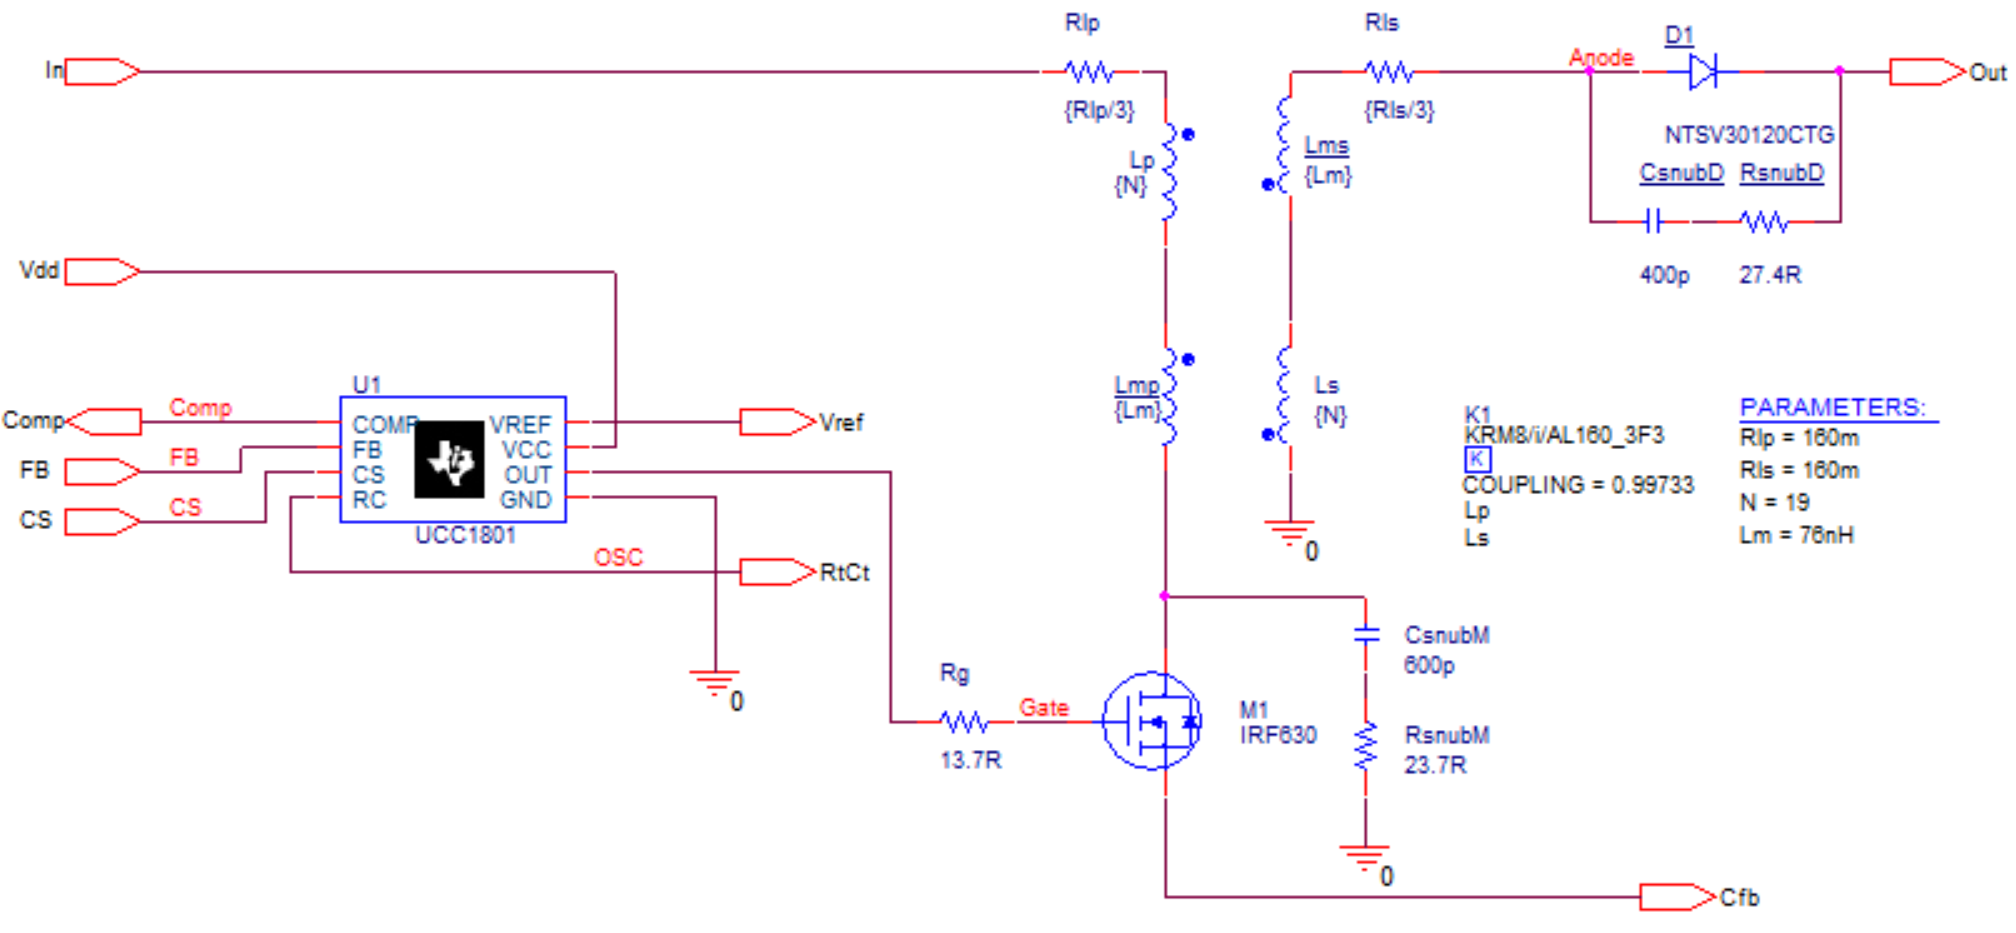
\includegraphics[max width=0.7\linewidth]{/tex/3iteration/billeder/Simulering/Simulering_power_diagram.PNG}
	\caption{Diagram for power modul med snubbere}
	\label{fig:simulering_diagram_snubber_3}
\end{figure}

\noindent Først måles MOSFET'ens drainspænding, i det tidspunk MOSFET'en går OFF, for at teste det primære snubber-kredsløb. Det er vist på figur~\ref{fig:simulering_snubber_MOSFET_3}. Her ses det, at svingningerne er blevet dæmpet ud, efter den første forventede svingning. Der kommer dog en lille anden svingning, som kommer da der er designet efter svingningerne aflæst i realiseringen, og ikke svingningerne aflæst i simuleringen for 2. iteration.  

\begin{figure}[H]
	\center
	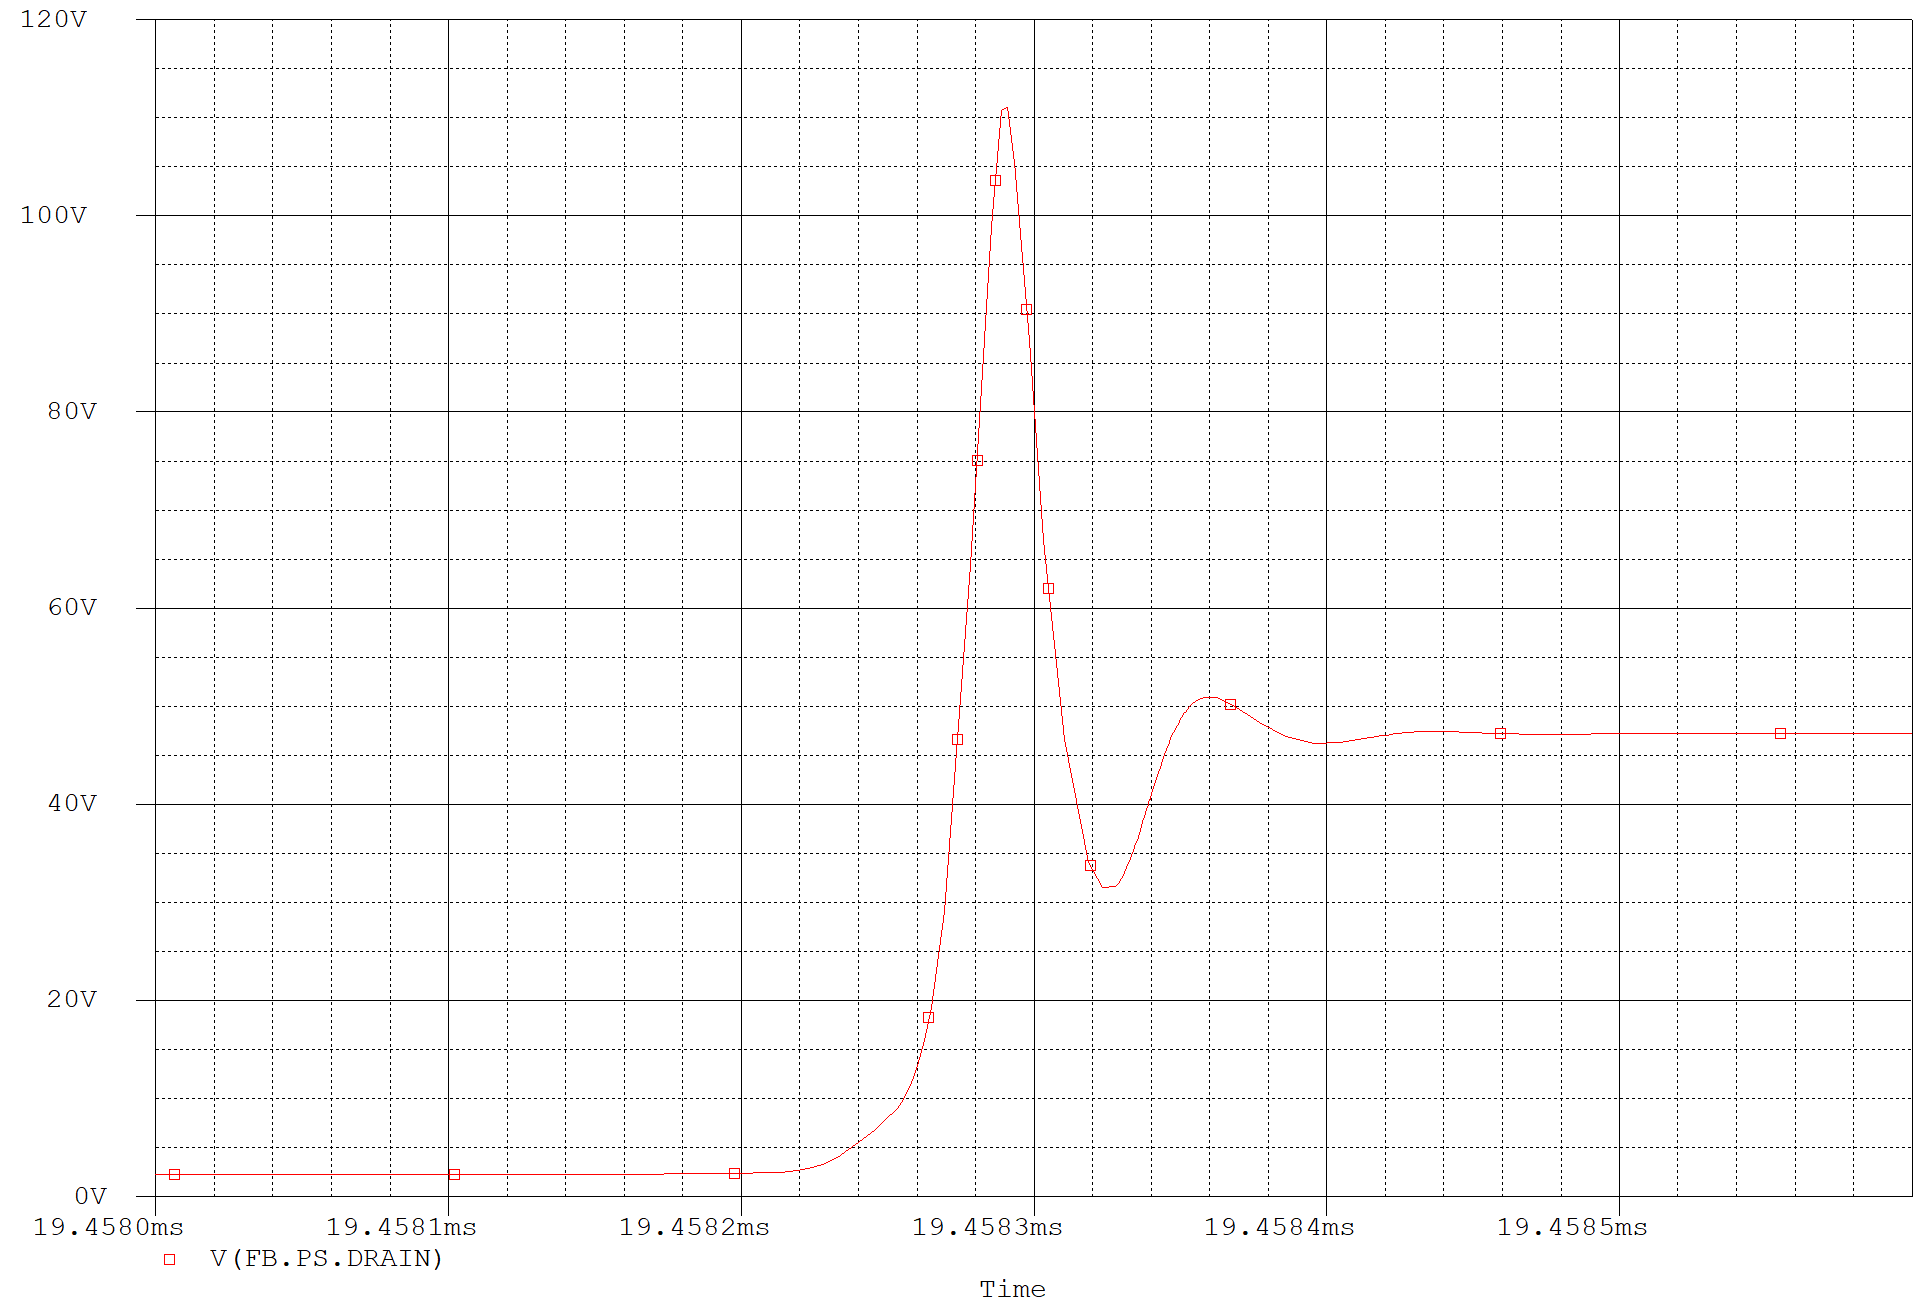
\includegraphics[max width=0.7\linewidth]{/tex/3iteration/billeder/Simulering/Simulering_snubber_MOSFET.PNG}
	\caption{Drain spænding efter snubber er tilføjet}
	\label{fig:simulering_snubber_MOSFET_3}
\end{figure}

\noindent Nu måles diodens anode spænding, i det tidspunkt MOSFET'en går ON, for at teste det sekundære snubber-kredsløb. Det er vist på figur~\ref{fig:simulering_snubber_diode_3}. Her ses det også, at snubber-kredsløbet har dæmpet de efterfølgende svingninger. Igen ses den lille anden svingning, da der er aflæst efter realiseringen.

\begin{figure}[H]
	\center
	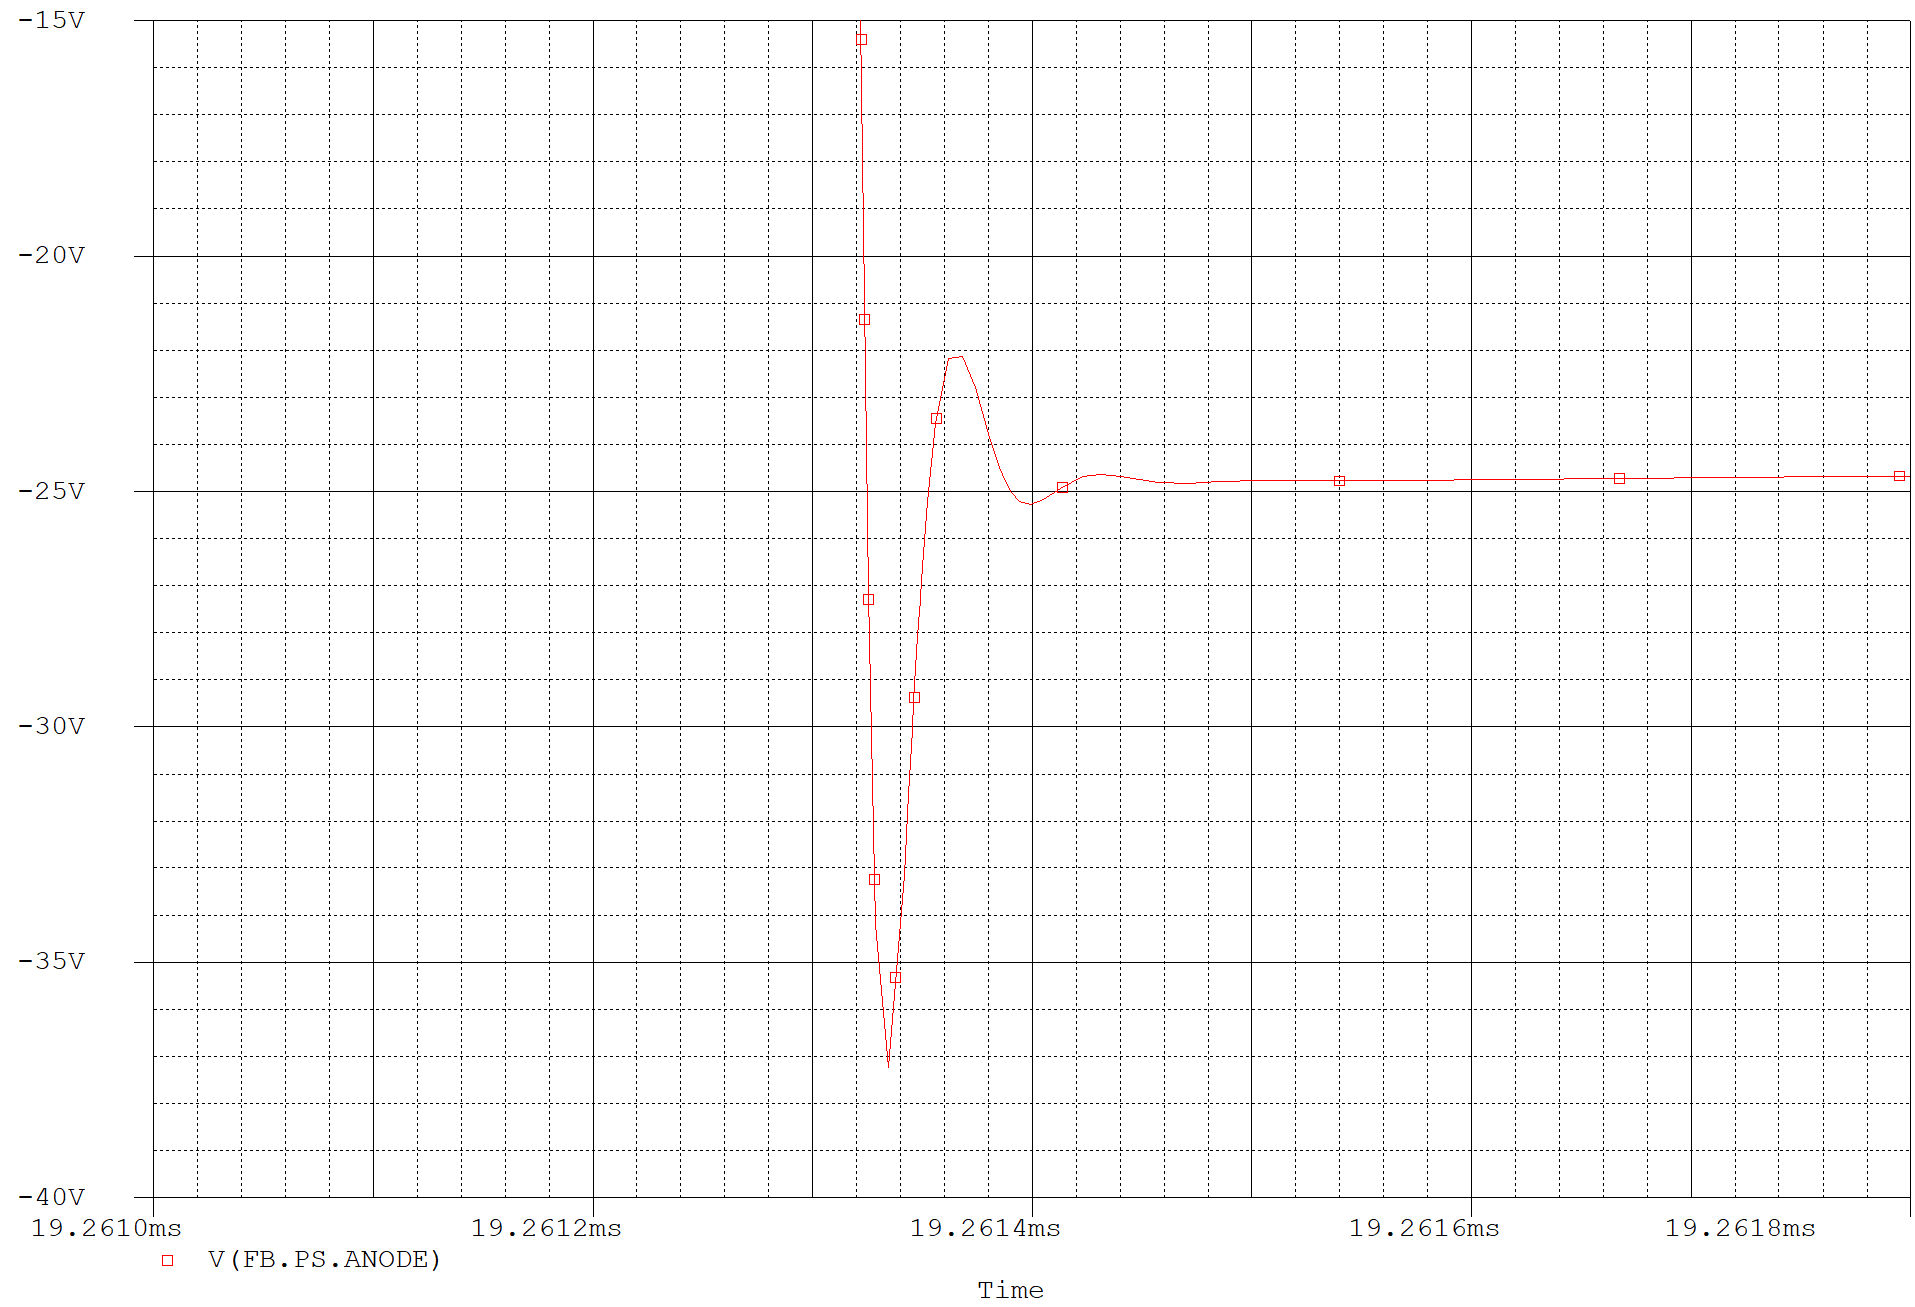
\includegraphics[max width=0.7\linewidth]{/tex/3iteration/billeder/Simulering/Simulering_snubber_diode.PNG}
	\caption{Anode spænding efter snubber er tilføjet}
	\label{fig:simulering_snubber_diode_3}
\end{figure}








%%% Simuleirng af optimering af udgangsfilter %%%

\subsection{Udgangsfilter}
Simulering af det optimerede udgangsfilter, gøres ved at modulere selvinduktionerne i ledningerne, som er en del af filteret. Kredsløbet for dette ses på figur~\ref{fig:diagram_udgangsfilter_3}. Her er filteret moduleret som de fire kondensatorer i parallel, og med selvinduktionerne på $30nH$ i ledningerne mellem dem. 

\begin{figure}[H]
	\center
	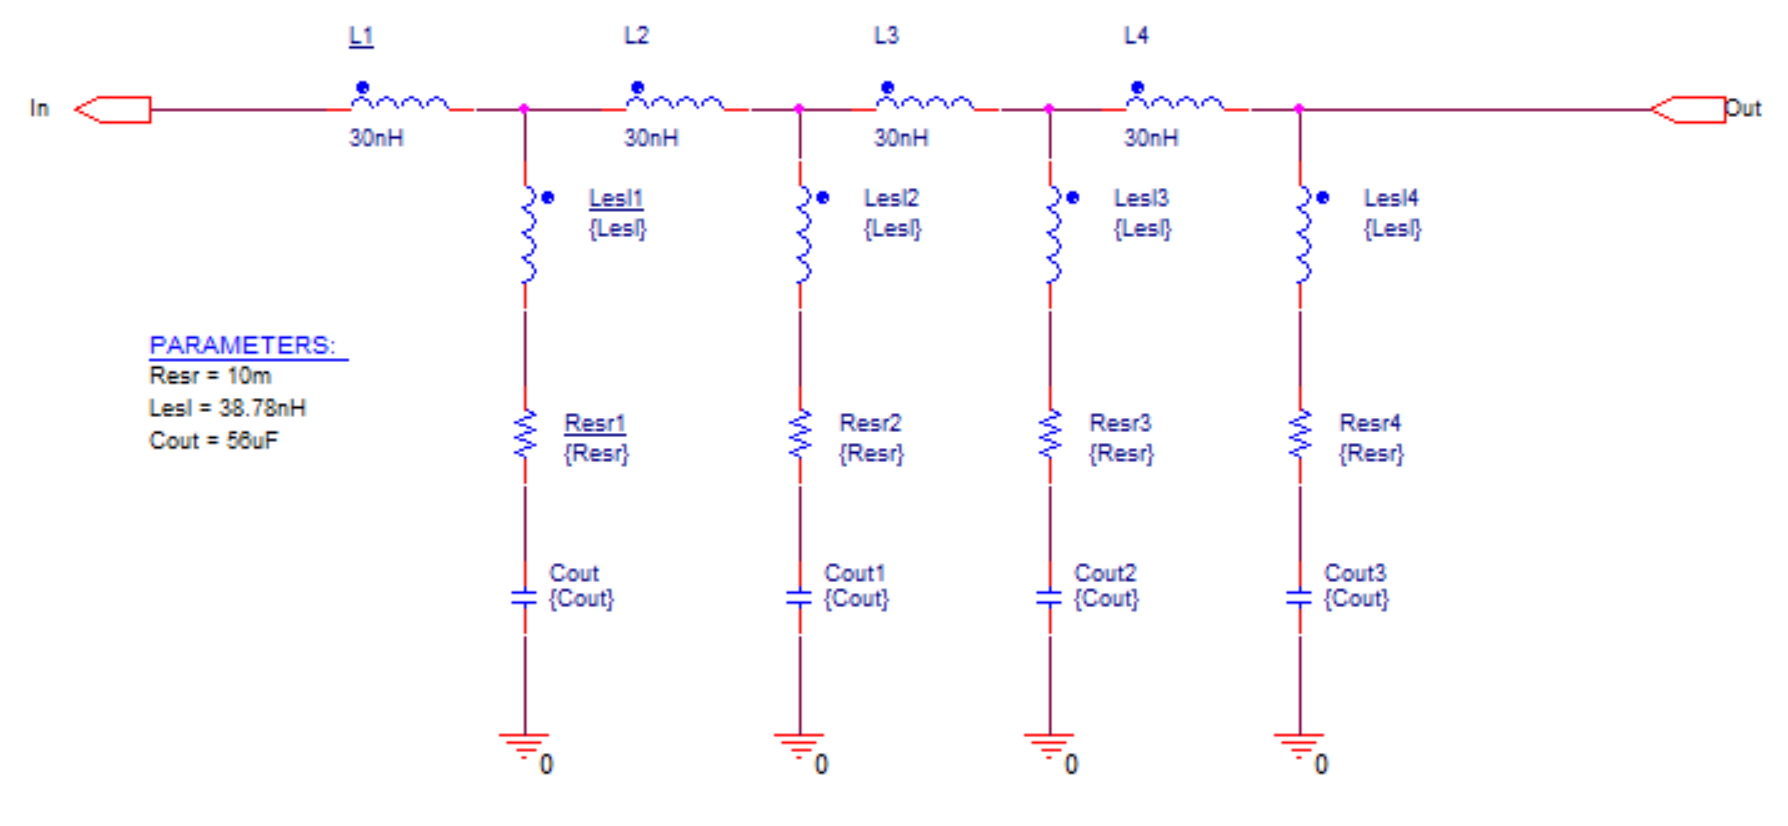
\includegraphics[max width=0.7\linewidth]{/tex/3iteration/billeder/Simulering/diagram_udgangsfilter.png}
	\caption{Diagram for udgangsfilter}
	\label{fig:diagram_udgangsfilter_3}
\end{figure}

\noindent Simuleringen er foretaget på figur~\ref{fig:simulering_udgangsfilter_U} og \ref{fig:simulering_udgangsfilter_M}. Her vises udgangssignalet før filteret på figur~\ref{fig:simulering_udgangsfilter_U}. Her aflæses der en spike på ca. $10V pk-pk$. Det er en større spike end ved realiseringen i 2. iteration, men viser at det er noget der skal filtreres væk. Figur~\ref{fig:simulering_udgangsfilter_M} viser signalet efter filteret. Her aflæses spiken til ca. $900mV pk-pk$. Det viser, at den teoretiske funktionalitet er opnået ved, at flytte udgangen til efter filteret. 

\begin{figure}[H]
	\center
	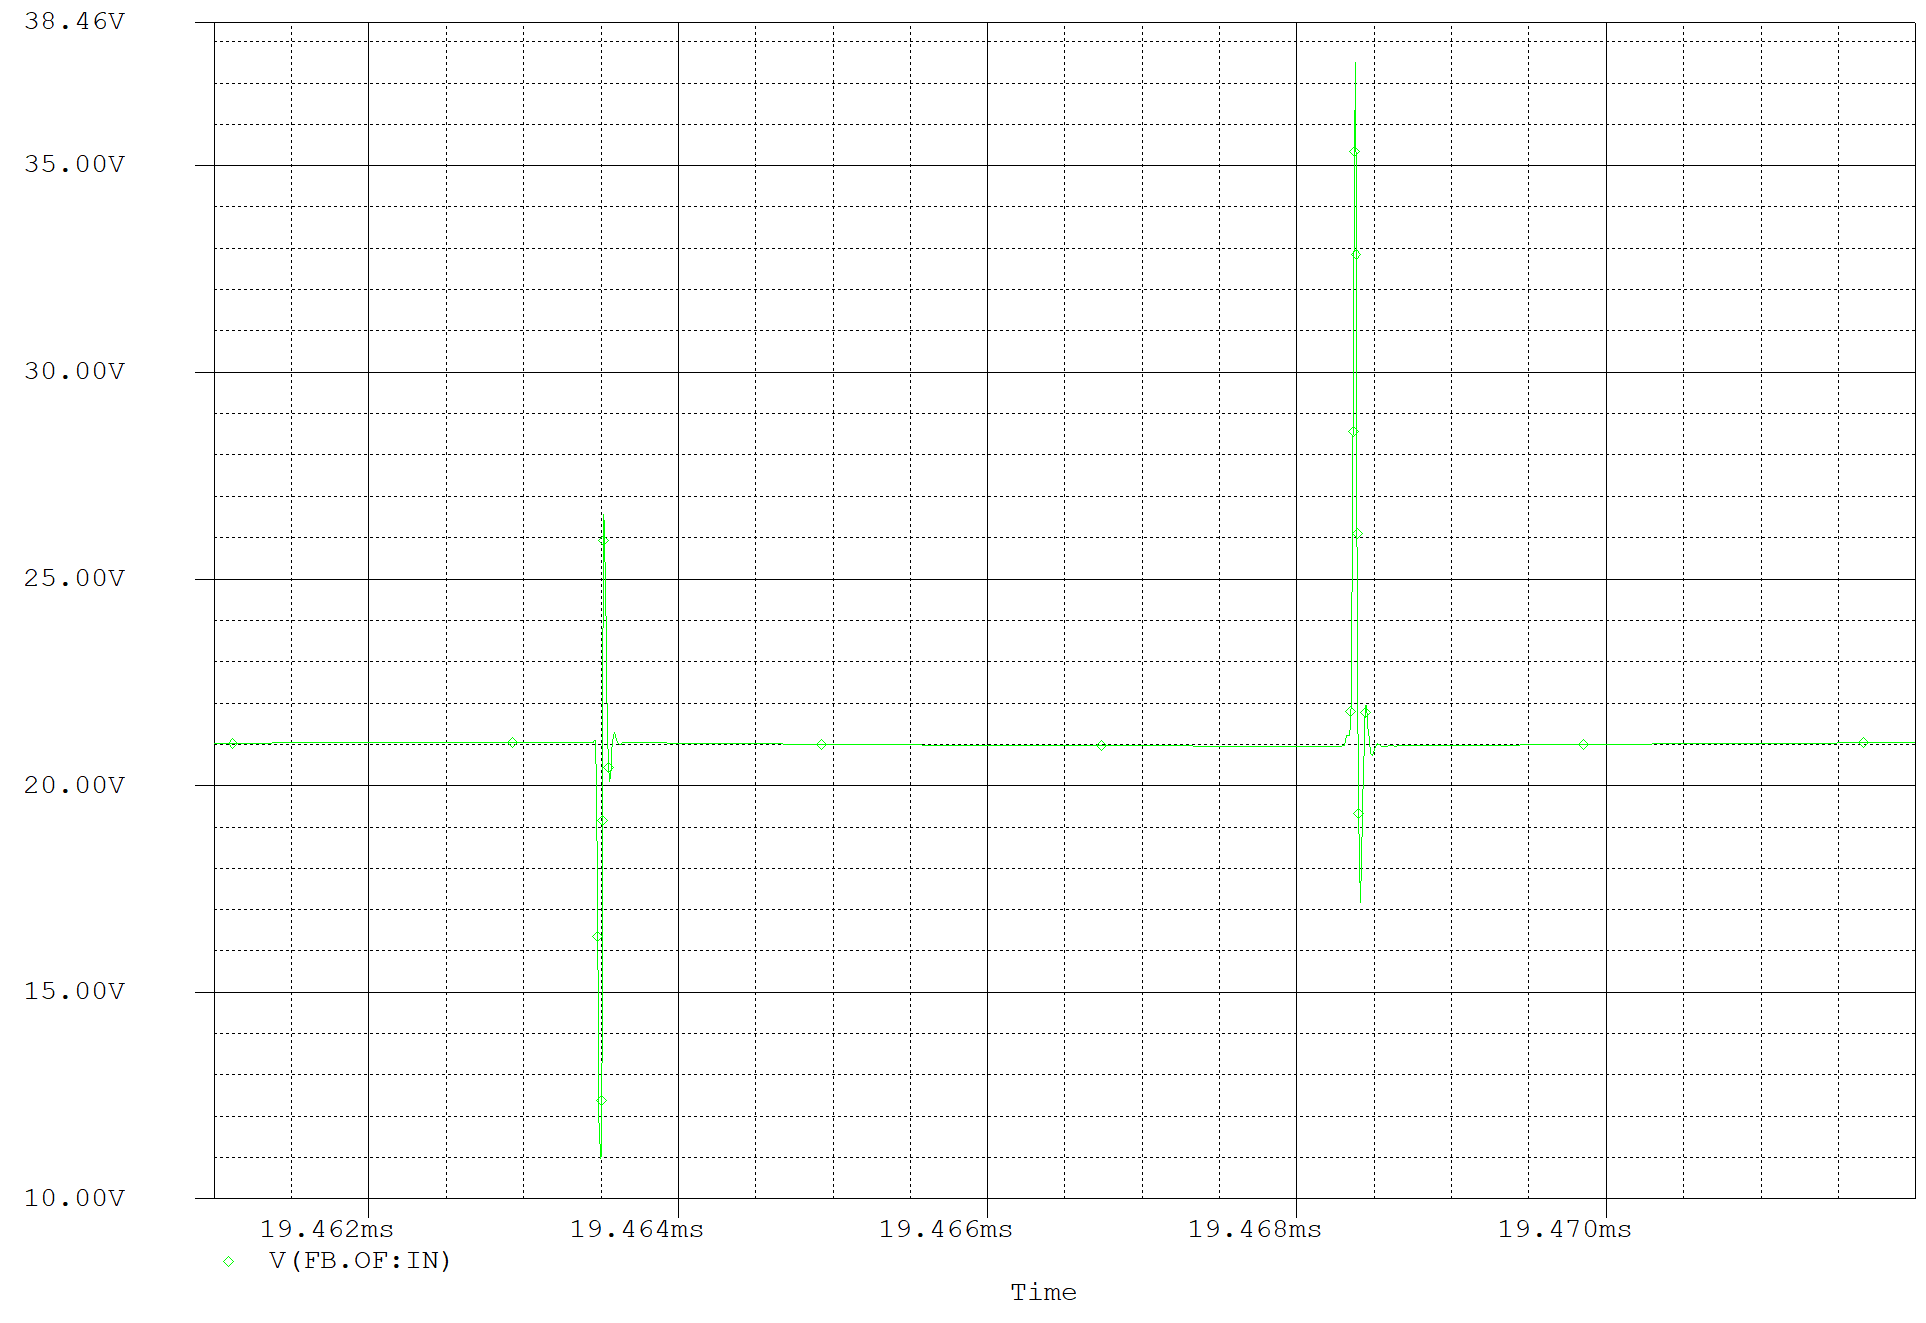
\includegraphics[max width=0.7\linewidth]{/tex/3iteration/billeder/Simulering/Simulering_udgangsfilter_U.png}
	\caption{Udgangssignal før filteret}
	\label{fig:simulering_udgangsfilter_U}
\end{figure}

\begin{figure}[H]
	\center
	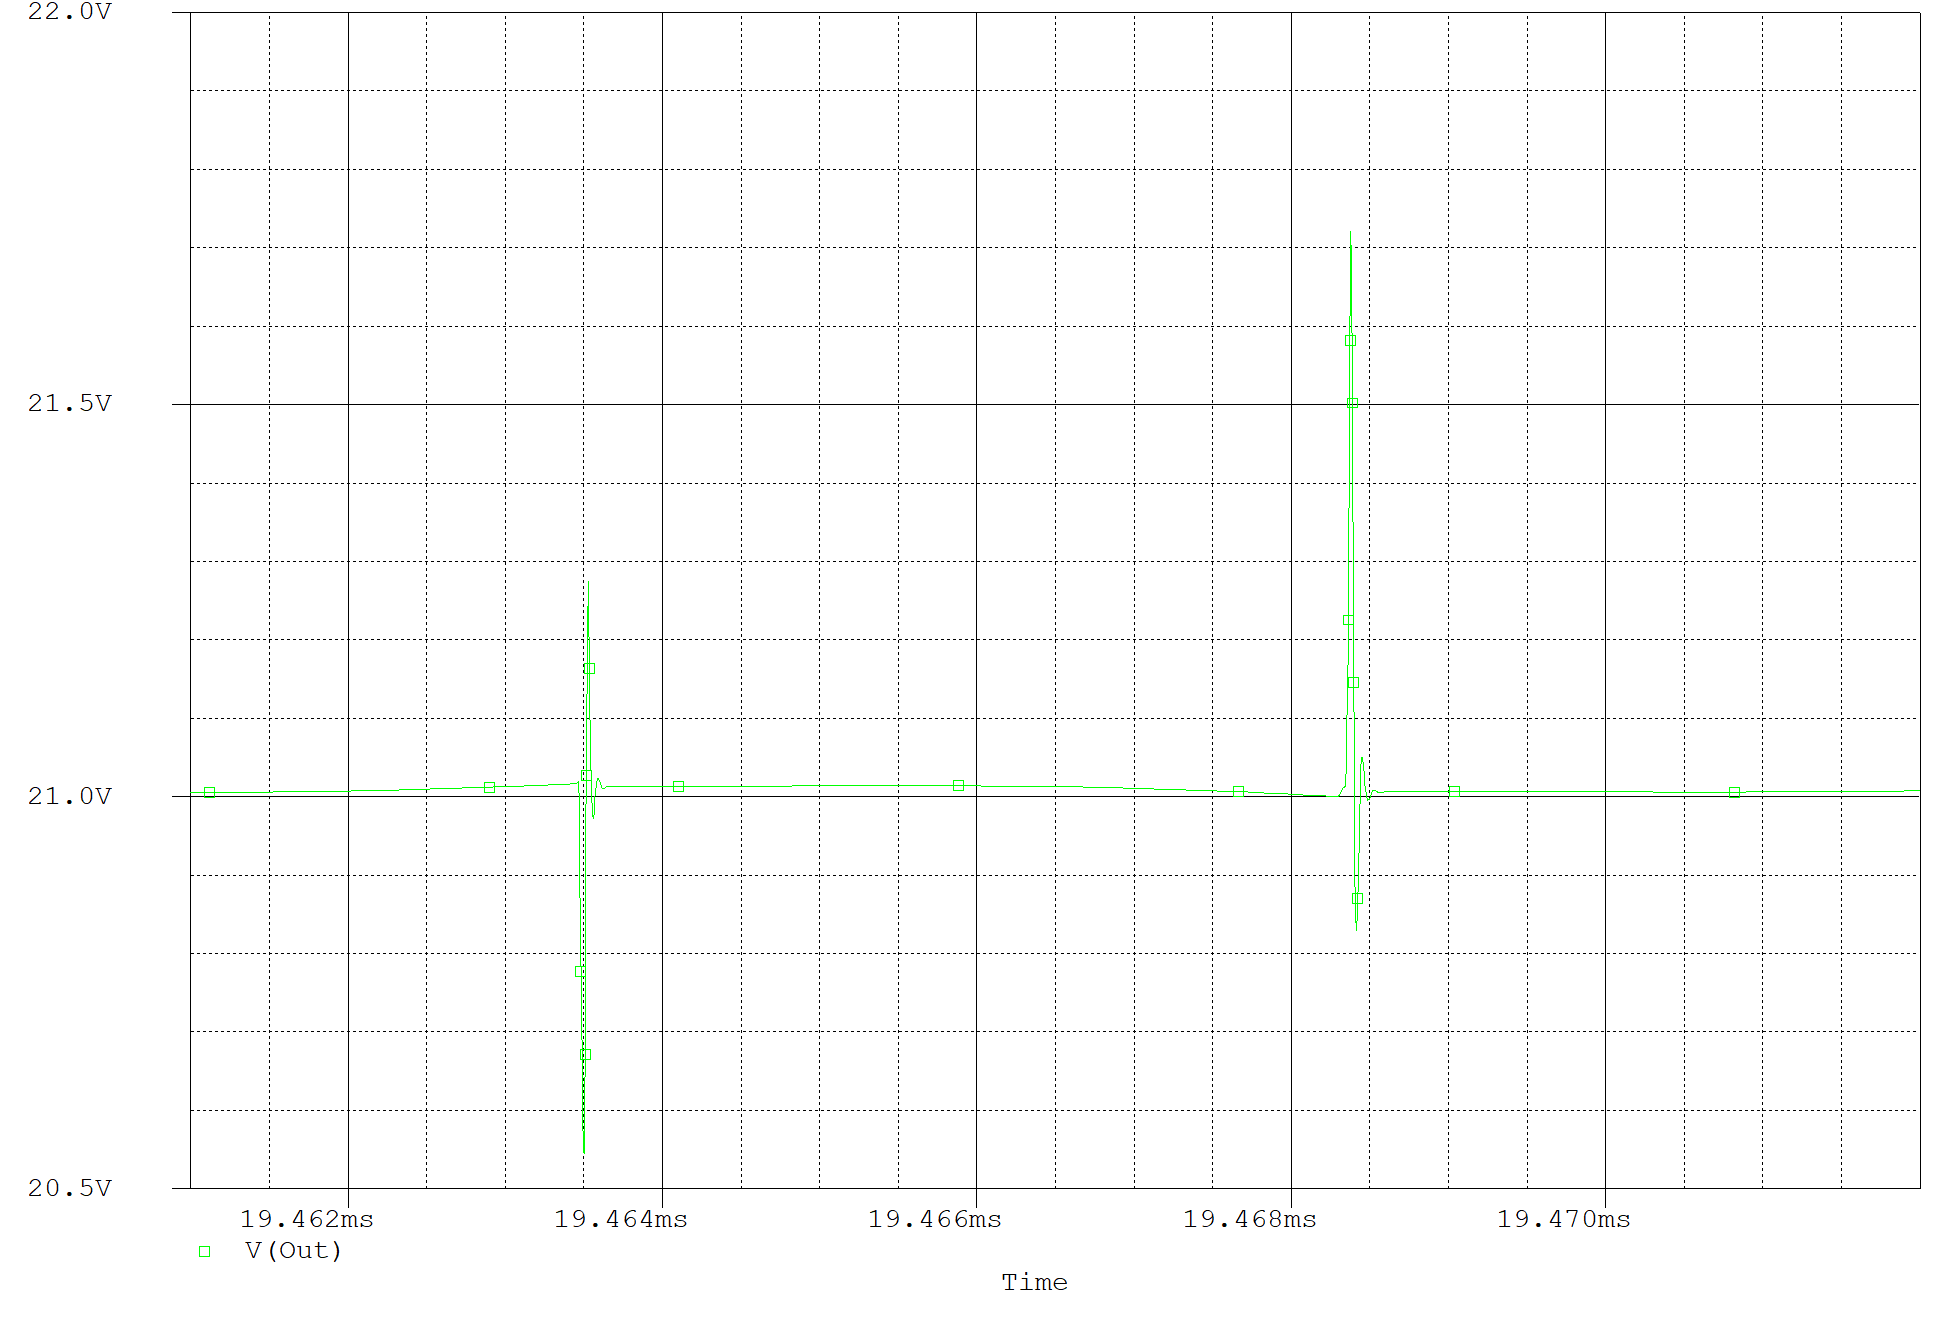
\includegraphics[max width=0.7\linewidth]{/tex/3iteration/billeder/Simulering/Simulering_udgangsfilter_M.png}
	\caption{Udgangssignal efter filteret}
	\label{fig:simulering_udgangsfilter_M}
\end{figure}


%%% Simulering for optimering af reguleringsloop %%%

\subsection{Gain-fase}
Simuleringen af systemets gain-fase karakteristik, udføres på samme måde som ved 2. iteration. Bode plot for fejlforstærkeren er vist på figur~\ref{fig:Simulering_error_op_amp_3}. Da knækfrekvensen for fejlforstærkeren ligger ved $132\hertz$, og der ikke kan simuleres med frekvenser lavere end $100\hertz$, er det svært at aflæse bode plottet. Det kan dog aflæses, at forstærkningen over $132^\circ$ ligger sig på ca. $8.6\decibel$. Derudover ses det at fasen stiger til $180^\circ$, derfor antages det, at fejlforstærkeren vil bidrage med det forventede faseløft på $90^\circ$. 

\begin{figure}[H]
	\center
	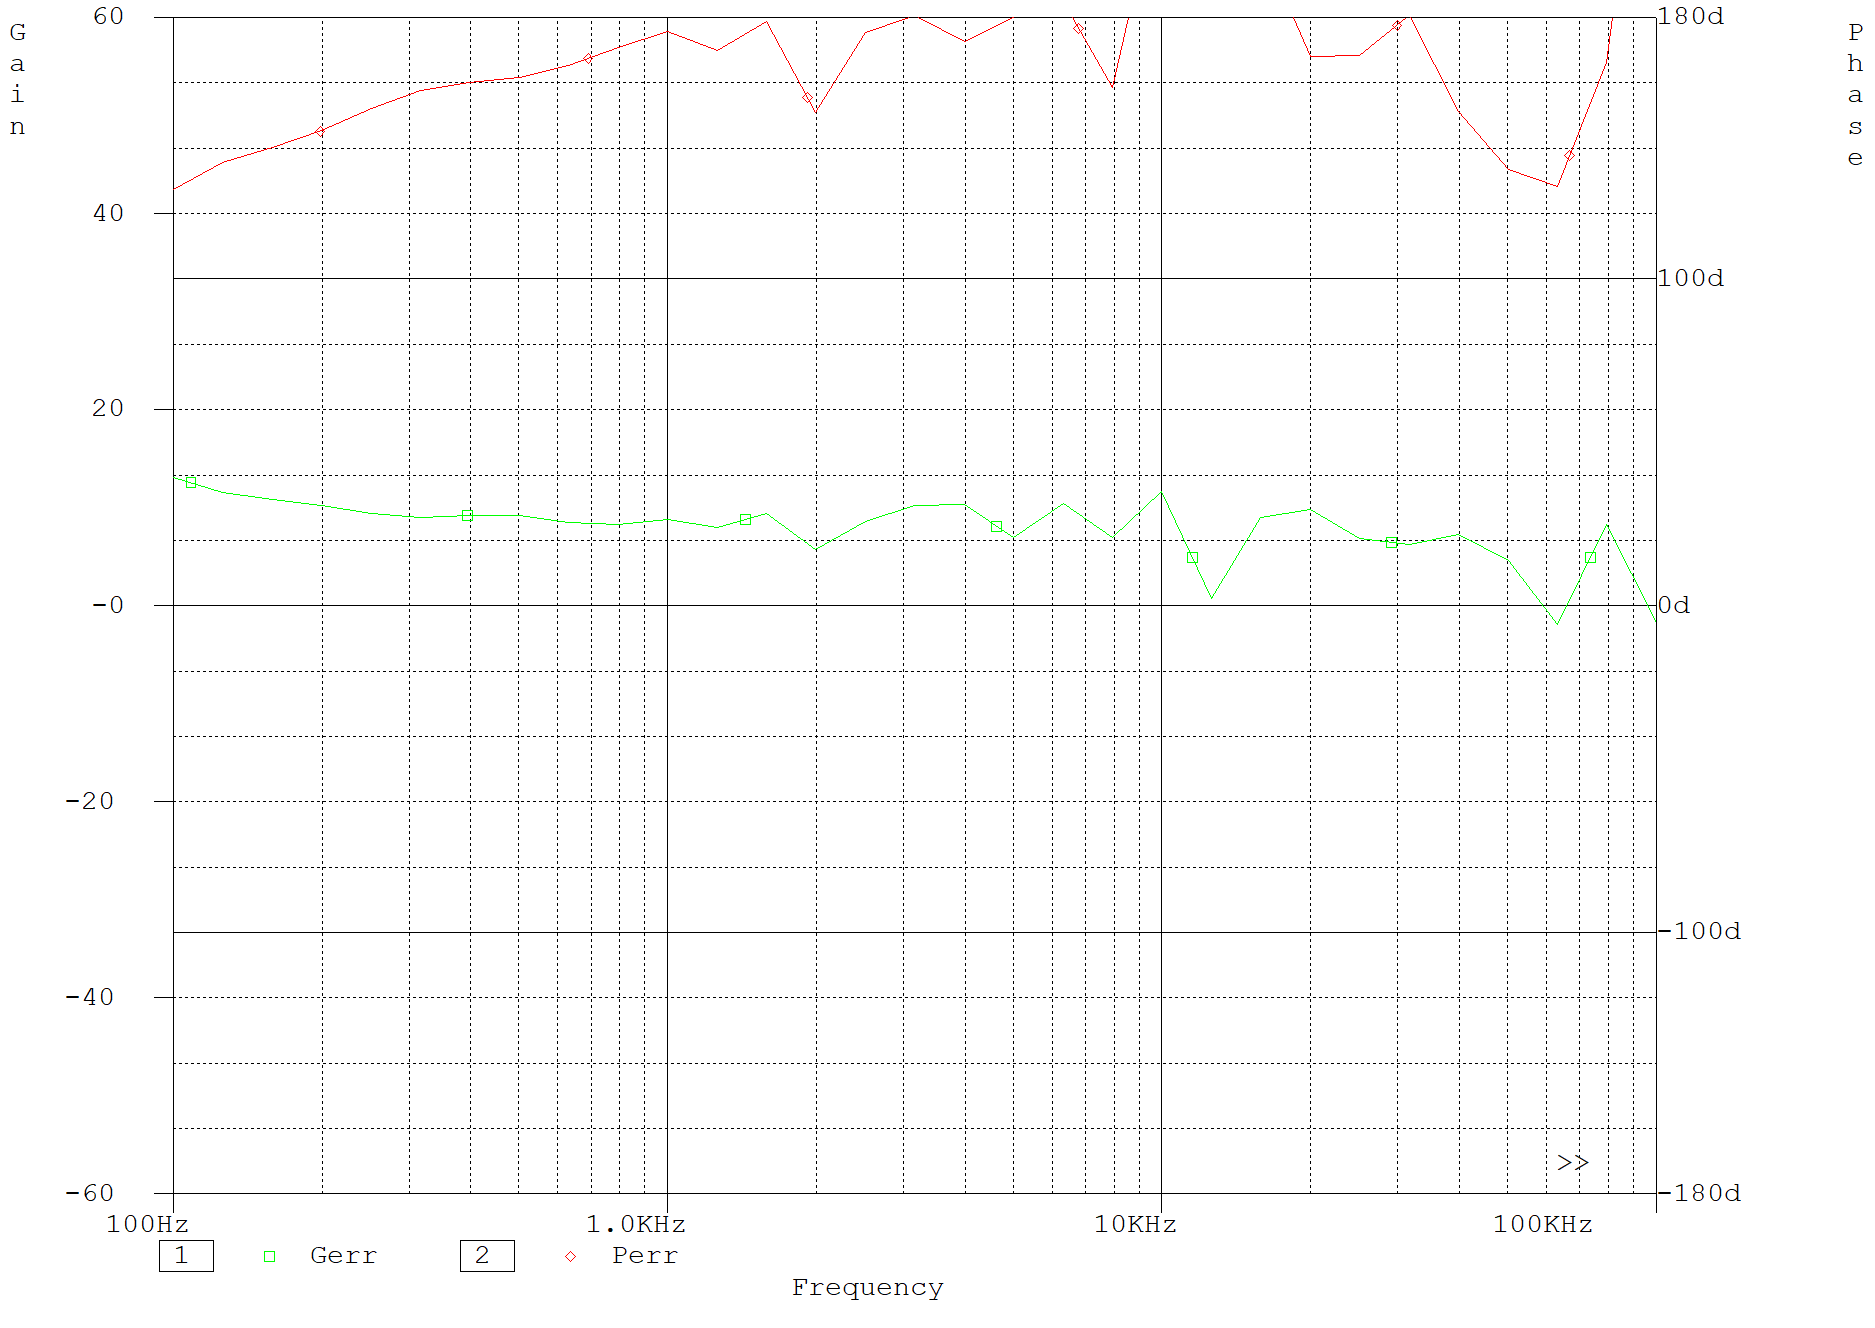
\includegraphics[max width=0.9\linewidth]{/tex/3iteration/billeder/Simulering/Simulering_error_op_amp.PNG}
	\caption{Simulering af fejlforstærkeren}
	\label{fig:Simulering_error_op_amp_3}
\end{figure}

\noindent Bode plottet for det samlede system er vist på figur~\ref{fig:Simulering_total_3}. Selvom simuleringen bliver usikker ved høje frekvenser, sker det så langt oppe i frekvens, at de relevante værdier akkurat kan aflæses. Gain-margin aflæses til ca. $10.2\decibel$, fase-margin aflæses til ca. $73.2^\circ$, og båndbredden aflæses til ca. $3.5k\hertz$. Ift. analysen passer både gain- og fasemargin, mens båndbredden ca. $400\hertz$ lavere end det forventede. 

\begin{figure}[H]
	\center
	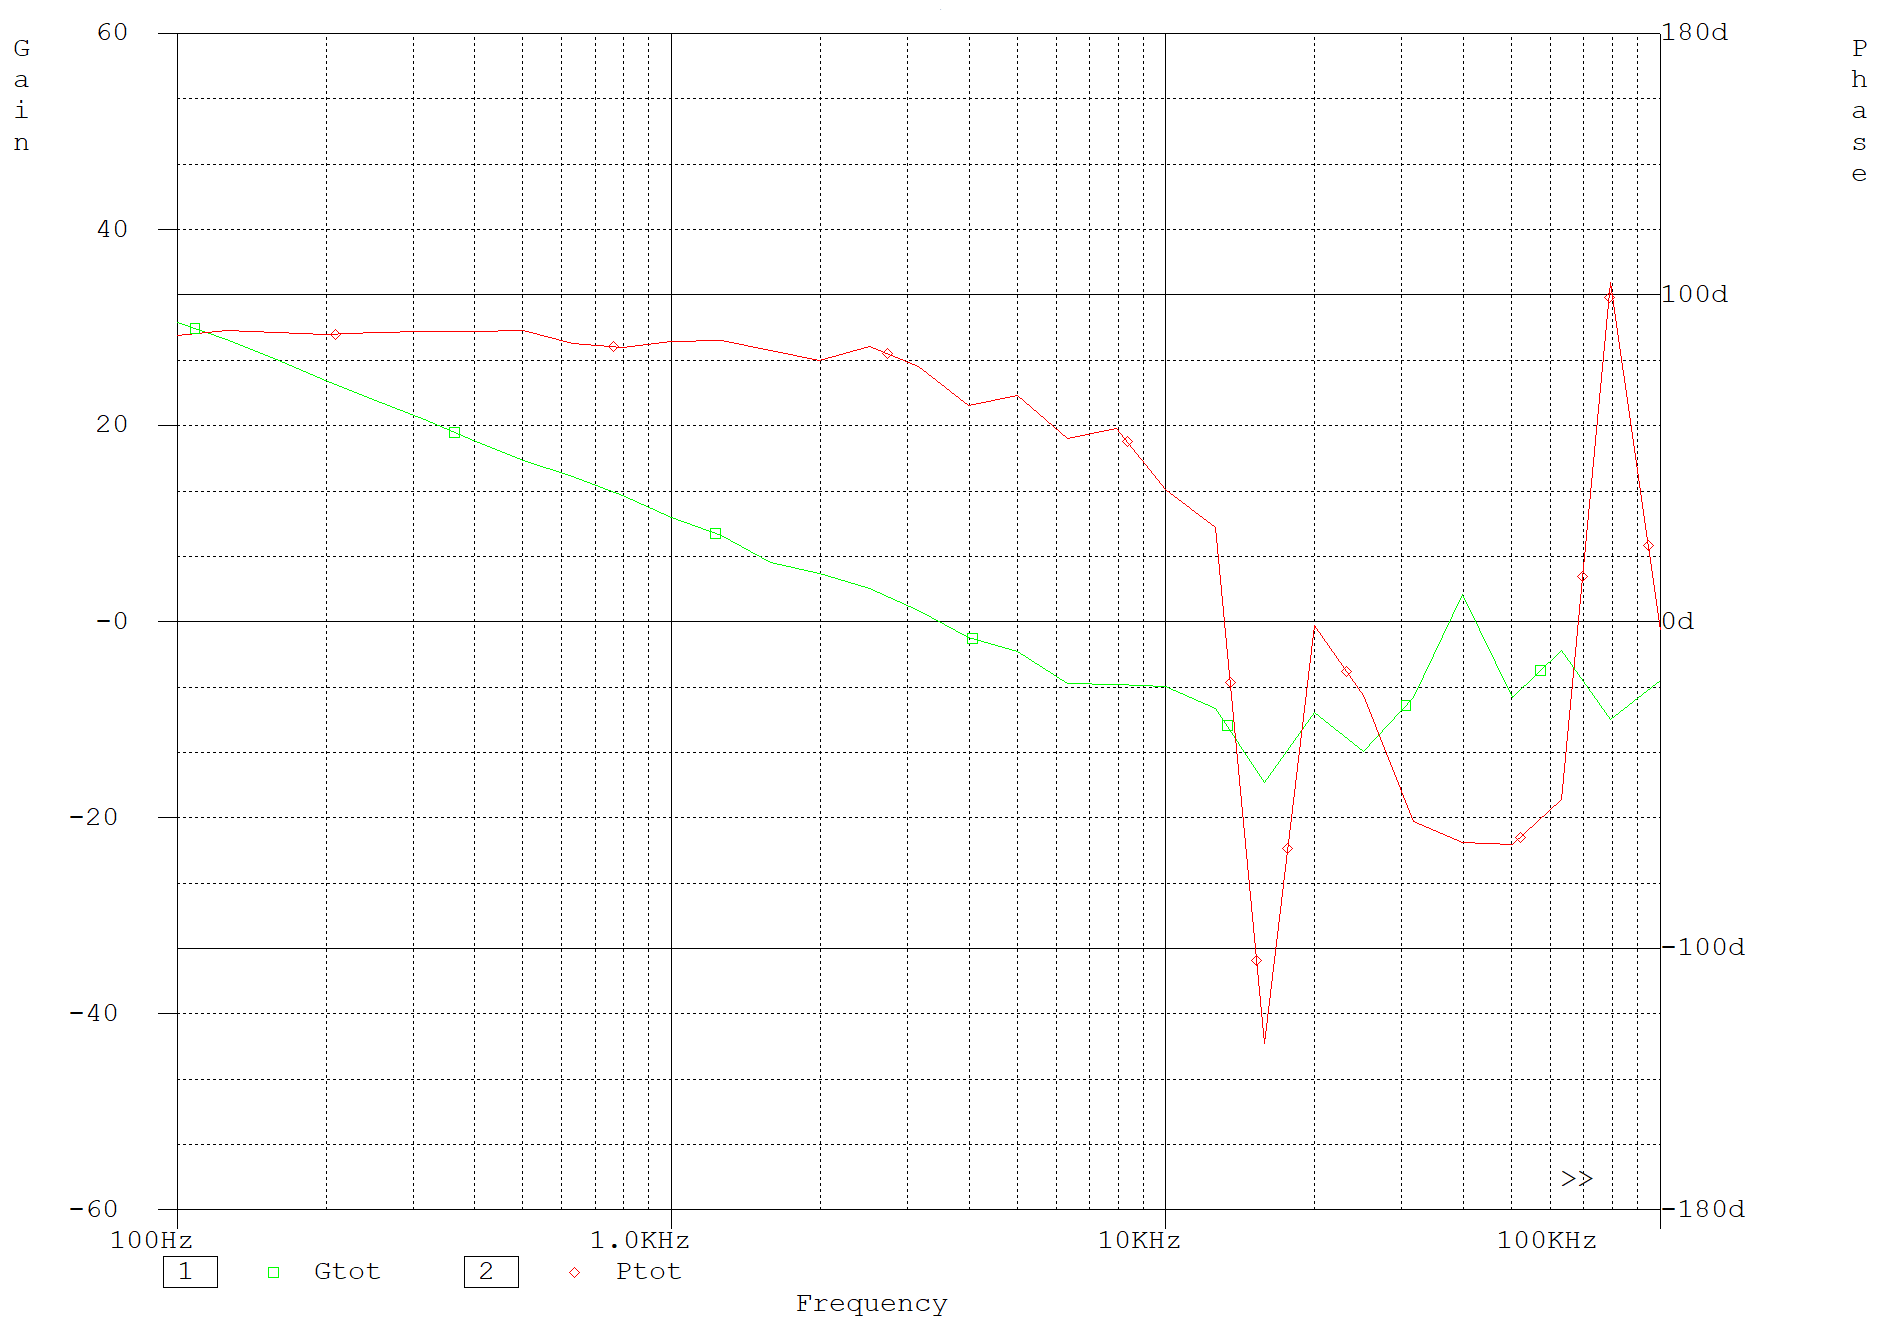
\includegraphics[max width=0.9\linewidth]{/tex/3iteration/billeder/Simulering/Simulering_total.PNG}
	\caption{Simulering af det samlede system}
	\label{fig:Simulering_total_3}
\end{figure}

\subsection{Load step}
Load steppet er i 3. iteration simuleret på samme måde, som det blev gjort under 2. iteration i sektion ~\ref{loadstep2ite}. Med en større båndbredde ændrer systemets loadstep. Derfor ser loadsteppet efter de nye gain-phase målinger ud som på ~\ref{fig:Loadstepsim2}
\begin{figure}[H]
	\center
	\includegraphics[max width=0.7\linewidth]{/tex/3iteration/billeder/simulering/Loadstep.PNG}
	\caption{Realiseret load step}
	\label{fig:Loadstepsim2}
\end{figure} 
Her ses det, at overshootet er blevet mindre. Det aflæses til ca. $300mV$ ved første dyk og $200mV$ ved stigningen. Selve reguleringstiden er blevet noget længere og aflæses til ca. $4ms$ for begge loads. 


\subsection{Tab}

\subsubsection{MOSFET}
\noindent Det nye simulerede samlede tab i MOSFET'en ses på figur~\ref{fig:simulering_power_MOSFET}. Simuleringen foregår på samme måde som ved sektion ~\ref{MOSFETsimtab}, hvor gate-modstanden i stedet er ændret til de $13.7\ohm$. Her aflæses den samlede afsatte effekt i MOSFET'en til ca. $3.2\watt$. 

\begin{figure}[H]
	\center
	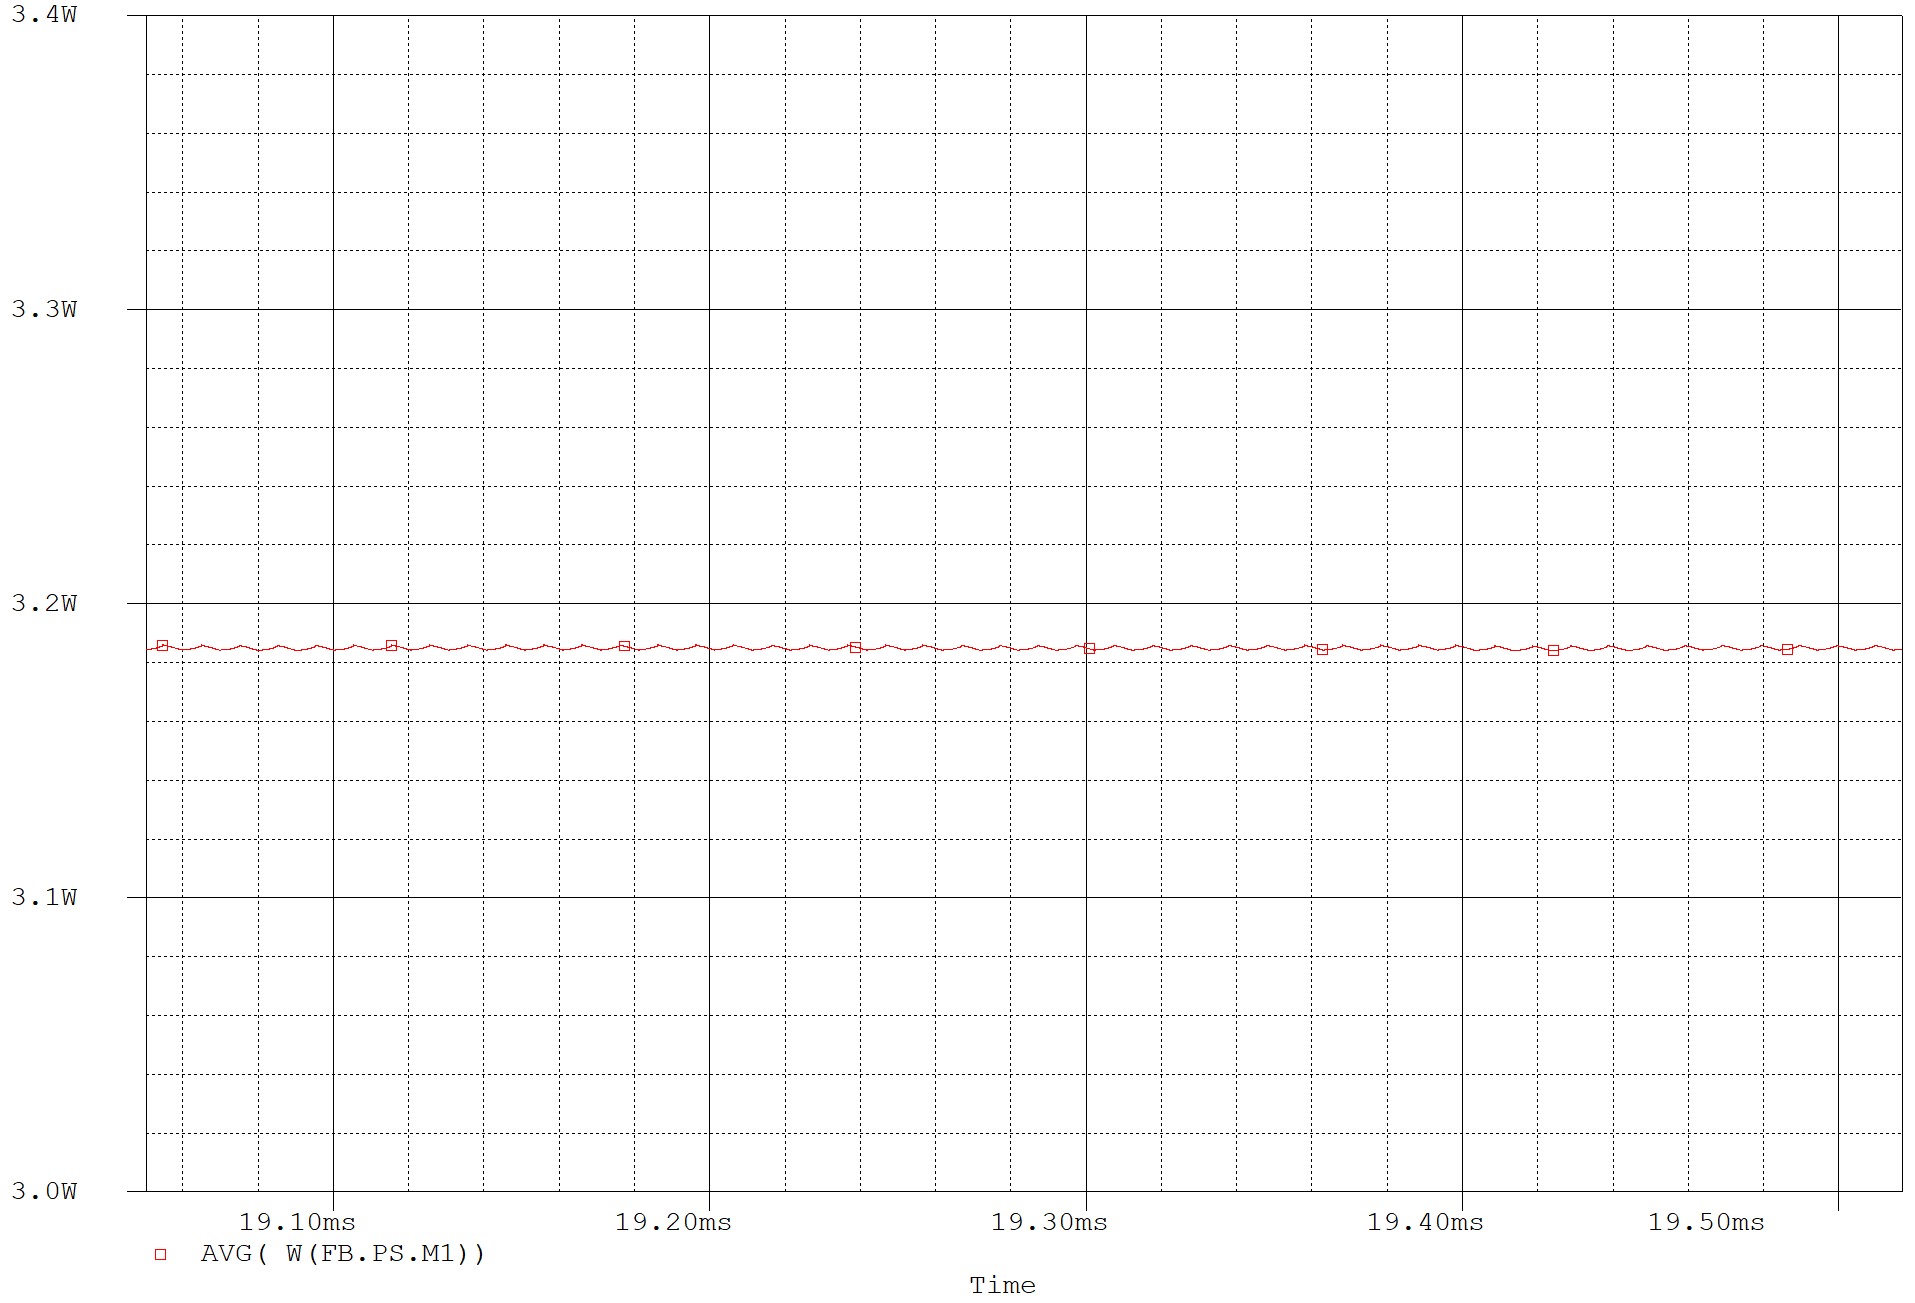
\includegraphics[max width=0.7\linewidth]{/tex/3iteration/billeder/Simulering/simulering_power_MOSFET.png}
	\caption{Simulering af effektafsættelse i MOSFET}
	\label{fig:simulering_power_MOSFET}
\end{figure}

\subsubsection{Snubber-kredsløb}
\noindent Tabet i snubber-kredsløbene simuleres ved, at kigge på tabene i snubber-modstandene, da det er her effekten bliver afsat. Figur~\ref{fig:simulering_power_snubber_MOSFET} viser effekten afsat i det primære snubber-kredsløb. Her aflæses effekten til $234m\watt$. Figur~\ref{fig:simulering_power_snubber_diode} viser effekten afsat i det sekundære snubber-kredsløb. Her aflæses effekten til $74m\watt$. 

\begin{figure}[H]
	\center
	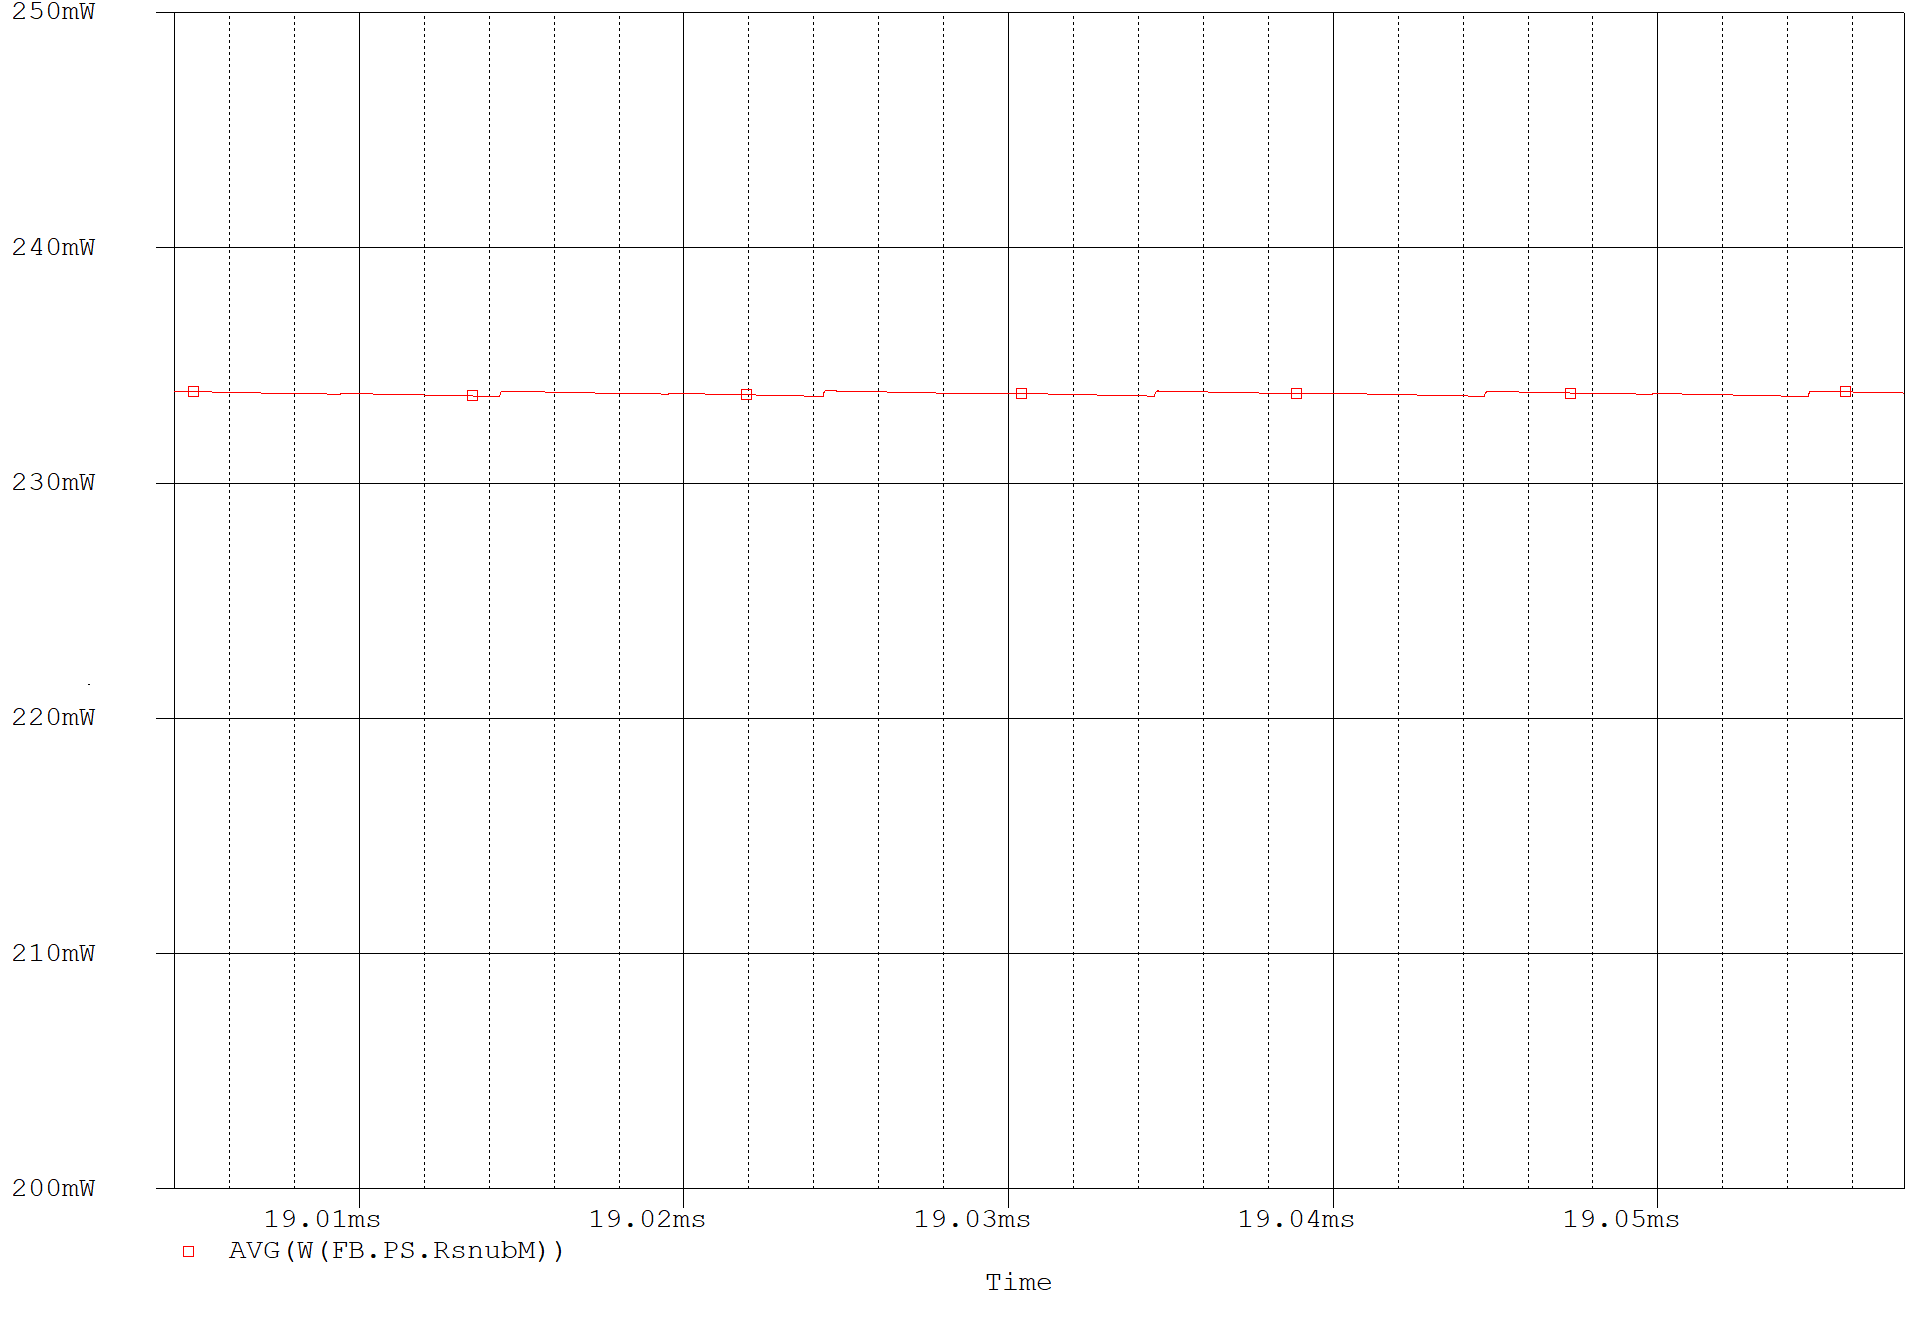
\includegraphics[max width=0.7\linewidth]{/tex/3iteration/billeder/Simulering/simulering_snubber_power_MOSFET.png}
	\caption{Simulering af effektafsættelse i det primære snubber-kredsløb}
	\label{fig:simulering_power_snubber_MOSFET}
\end{figure}

\begin{figure}[H]
	\center
	\includegraphics[max width=0.7\linewidth]{/tex/3iteration/billeder/Simulering/Simulering_snubber_power_diode.png}
	\caption{Simulering af effektafsættelse i det sekundære snubber-kredsløb}
	\label{fig:simulering_power_snubber_diode}
\end{figure}

\subsubsection{Oversigt over simuleret tab}
\begin{table}[H] 			
	\centering
	\begin{tabularx}{\textwidth}{|X|l|l|}
		\hline
		\textbf{\large Komponent} & \multicolumn{2}{|l|}{\textbf{\large Tab}} \\ \hline
		& A & S	\\ \hline
		\textbf{Transformator samlet} & $1.46\watt$ & $1.62\watt$ \\ \hline 
		Kernetab & $366m\watt$ & $311m\watt$ \\ \hline
		Kobbertab & $1.09\watt$ & $1.31\watt$ \\ \hline
		& &	\\ \hline
		\textbf{MOSFET samlet} & $2.54\watt$ & $3.2\watt$ \\ \hline
		Conduction-tab & $1.06\watt$ & 	\\ \hline
		Switch-tab & $1.48\watt$ & 		\\ \hline
		& &	\\ \hline
		\textbf{Diode} & $1.13\watt$ & $1.47\watt$ \\ \hline
		& &	\\ \hline
		\textbf{CS modstands tab} & $1.52\watt$ & $2.03\watt$ \\ \hline
		& &	\\ \hline
		\textbf{Snubber-kredsløb} & $220.9m\watt$ & $308m\watt$ \\ \hline
		Primær snubber	& $132.5m\watt$	& $234m\watt$		\\ \hline
		Sekundær snubber &	$88.4m\watt$ &	$74m\watt$		\\ \hline
		& &	\\ \hline
		\textbf{Total tab} & $6.87\watt$ & $8.63\watt$ \\ \hline
	\end{tabularx}
	\caption{Oversigt over analyseret og simuleret tab}
	\label{tab:simulering_tab_3}
\end{table}

Figur~\ref{fig:simulering_power_samlet} viser en simulering af converterens indgangseffekt(grøn) og udgangseffekt(rød). Indgangseffekten er aflæst til $61.4\watt$, og udgangseffekten er aflæst til $52.7\watt$. Differensen på dette er det samlede effekttab i converteren, som er regnet til $8.7\watt$. Det viser, der er taget højde for de dominerende tab i tabsberegningerne. 

\begin{figure}[H]
	\center
	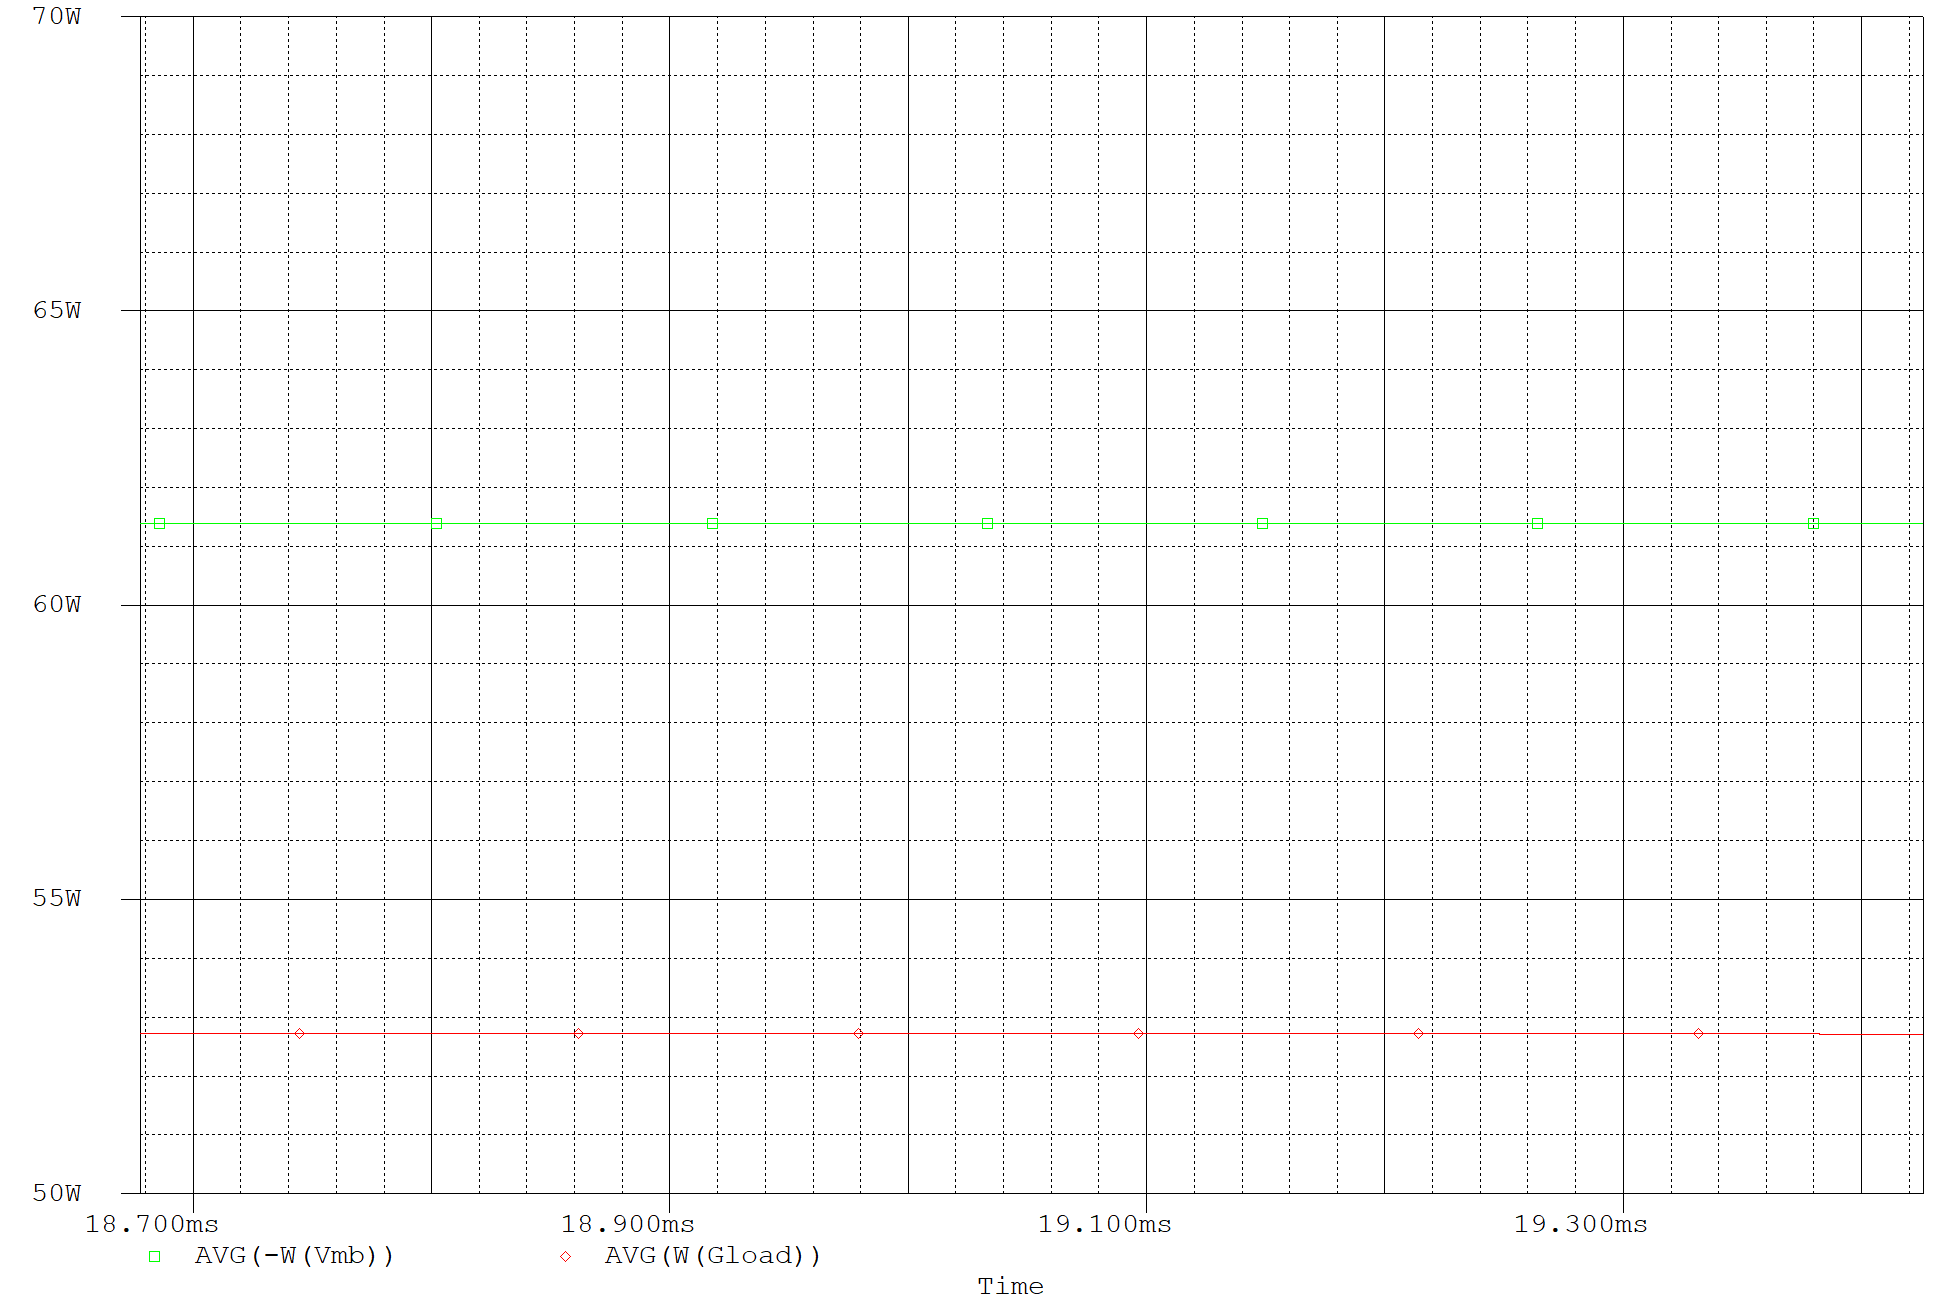
\includegraphics[max width=0.7\linewidth]{/tex/3iteration/billeder/Simulering/simulering_samlet_tab.png}
	\caption{Simulering af indgang- og udgangseffekt}
	\label{fig:simulering_power_samlet}
\end{figure}

\clearpage

\section{Realisering}
I det følgende afsnit vil de optimerede, og nye kredsløb realiseres. Det indebærer en optimering af switch-tiden og current-sense filteret, samt udvikling af snubber-kredsløb til både primær og sekundær siden af transformatoren. Det nye diagram for 3. iteration ses på figur~\ref{fig:samlet_opstilling}. Her er den største ændring ift. 2. iteration, der er indsat snubber-kredsløb over MOSFET og diode.

\begin{figure}[H]
	\center
	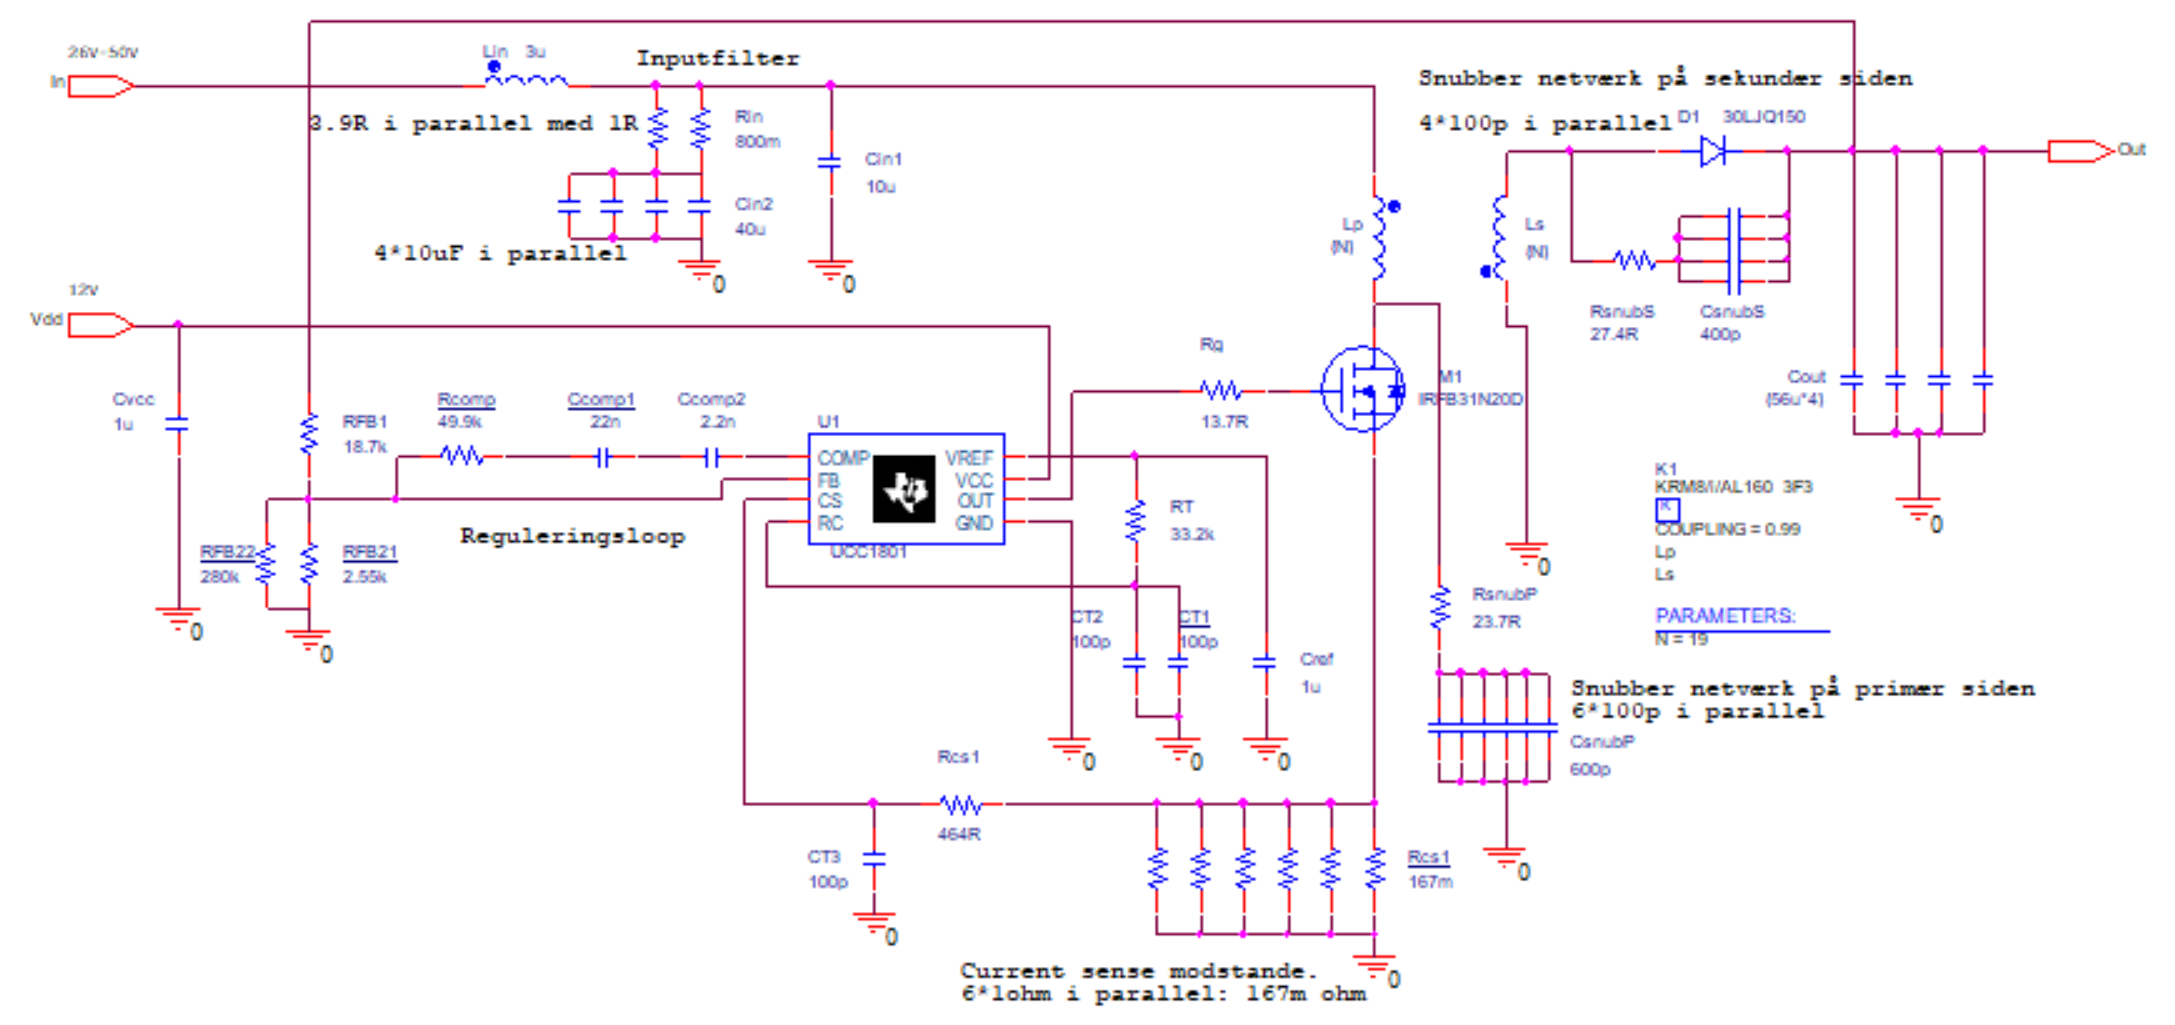
\includegraphics[max width=1.2\linewidth, angle=-90]{/tex/3iteration/billeder/Realisering/samlet_opstilling.png}
	\caption{Schematic overblik for 3. iteration}
	\label{fig:samlet_opstilling}
\end{figure}


%%% Realisering for optimering af gate-modstand %%%


\subsection{Switch-tid}
Implementeringen af den optimerede switch-tid testes ved, at måle MOSFET'ens gate signal. Det signal er vist på figur~\ref{fig:realisering_switch_tid_3}, hvor kanal 1 er MOSFET'ens drain, og kanal 2 er MOSFET'ens gate. Her aflæses switch-tiden til ca. $40ns$. Resultaterne fo analysen, simulering og realiseringen indføres i tabel~\ref{tab:resultat_switch_tid_3}. Her er simuleringen dog foretaget med en anden MOSFET.

\begin{table}[H] 			
	\centering
	\begin{tabularx}{\textwidth}{|X|c|c|c|}
		\hline
		\textbf{Tid} & \multicolumn{3}{|c|}{\textbf{Switch-tid}} 										\\ \hline
		& A & S & R 									\\ \hline
		$T_{ch}$ & $37.2ns$ & $29.4ns$ & $40ns$ 											\\ \hline 
		
	\end{tabularx}
	\caption{Resultater for analyse, simulering og realisering af switch-tid}
	\label{tab:resultat_switch_tid_3}
\end{table}

\begin{figure}[H]
	\center
	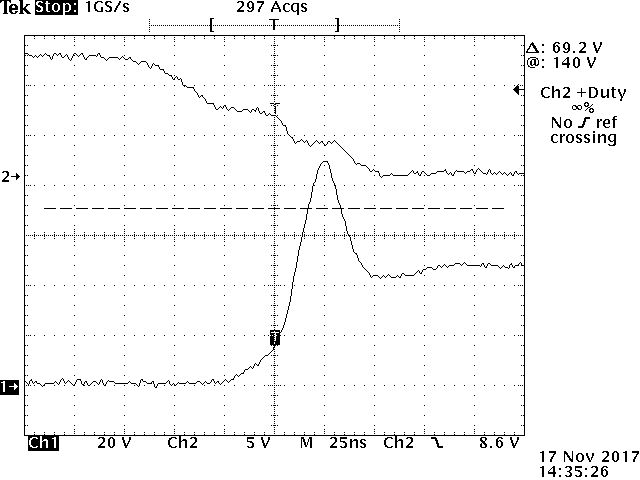
\includegraphics[max width=0.7\linewidth]{/tex/3iteration/billeder/Realisering/Realisering_switch_tid.png}
	\caption{Realisering af switch-tid for MOSFET - 3. iteration}
	\label{fig:realisering_switch_tid_3}
\end{figure}

%%% Realisering af optimering af current-sense filter %%%

\subsection{Current-sense filter}
For at teste optimeringen af current-sense filteret, måles signalet både før og efter filteret. Det filtrerede signal ses på figur~\ref{fig:Realisering_cs_M_3}, hvor kanal 1 viser current-sense signalet, og kanal 2 viser MOSFET'ens gate. Dette viser der opnået et filter med stort set rette flanker, og dermed en meget hurtigere stigetid. Figur~\ref{fig:Realisering_cs_M_zoom_3} viser current-sense signalet, hvor der er zoomet ind på flanken. Her aflæses stigetiden til ca. $100ns$. Samtidig ses det lille overshoot, som også kom ved simuleringen. Det viser der er opnået en optimal stigetid i filteret. Resultaterne for analyse, simulering og realisering er indført i tabel~\ref{label}.

\begin{table}[H] 			
	\centering
	\begin{tabularx}{\textwidth}{|X|c|c|c|}
		\hline
		\textbf{Tid} & \multicolumn{3}{|c|}{\textbf{Switch-tid}} 										\\ \hline
		& A & S & R 									\\ \hline
		$T_{r}$ & $100ns$ & $85ns$ & $100ns$ 										\\ \hline 
	\end{tabularx}
	\caption{Resultater for analyse, simulering og realisering af current-sense filter}
	\label{tab:resultat_cs_filter_3}
\end{table}


\begin{figure}[H]
	\center
	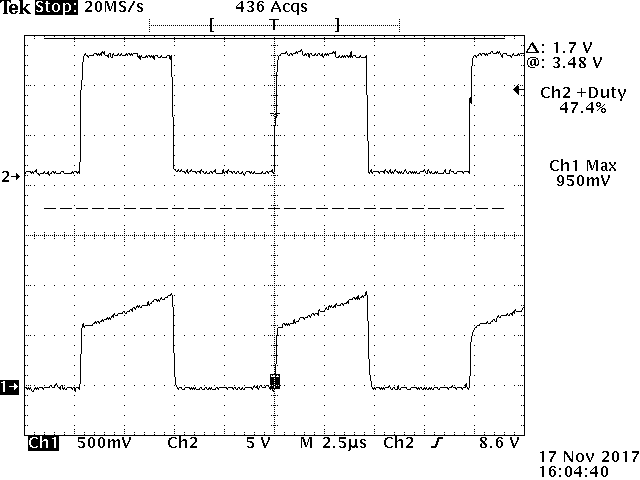
\includegraphics[max width=0.7\linewidth]{/tex/3iteration/billeder/Realisering/Realisering_cs_M.png}
	\caption{Realisering af optimering af current-sense signal efter filtrering}
	\label{fig:Realisering_cs_M_3}
\end{figure}

\begin{figure}[H]
	\center
	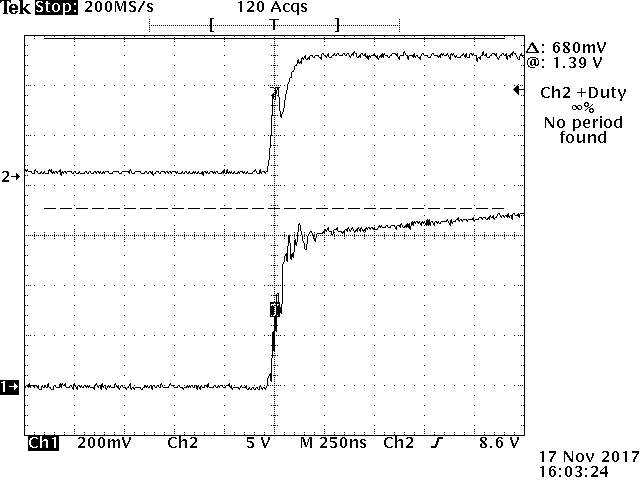
\includegraphics[max width=0.7\linewidth]{/tex/3iteration/billeder/Realisering/Realisering_cs_M_zoom.png}
	\caption{Realisering af optimering af current-sense signal efter filtrering - zoom}
	\label{fig:Realisering_cs_M_zoom_3}
\end{figure}

%%% Realiseirng for design af snubber-kredsløb til MOSFET og diode %%%

\subsection{Snubber-kredsløb}
For at teste realiseringen af snubber-kredsløbene måles MOSFET'ens drain spænding og diodens andode spænding. Først testes snubberen på primærsiden. Figur~\ref{fig:realiseirng_snubber_MOSFET_3} viser MOSFET'ens drain spænding. Her ses det, at den ønskede funktionalitet af den primære snubber er opnået. Signalet tager en enkelt svingning, og falder derefter til ro. Figur~\ref{fig:realiseirng_snubber_diode_3}, viser samme diodens anode spænding. Her ses det, at funktionalitet også er opnået ved det sekundære snubber-kredsløb. 

\begin{figure}[H]
	\center
	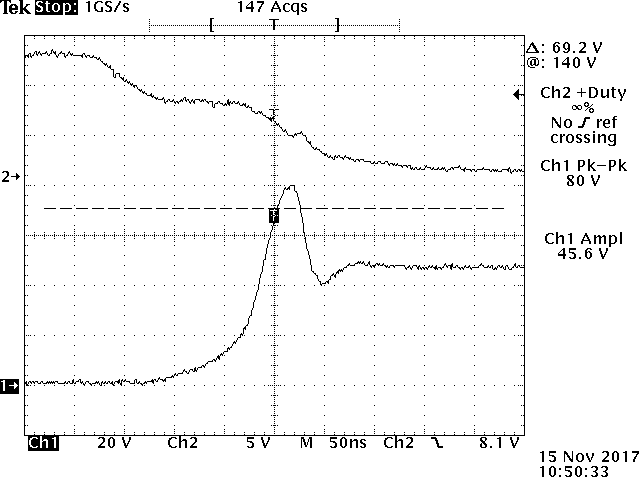
\includegraphics[max width=0.7\linewidth]{/tex/3iteration/billeder/Realisering/Realisering_snubber_MOSFET.PNG}
	\caption{Drain spænding efter snubber er tilføjet}
	\label{fig:realiseirng_snubber_MOSFET_3}
\end{figure} 

\begin{figure}[H]
	\center
	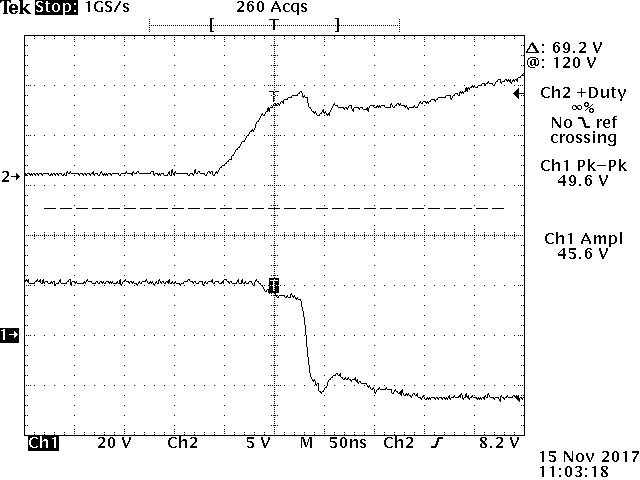
\includegraphics[max width=0.7\linewidth]{/tex/3iteration/billeder/Realisering/Realisering_snubber_diode.PNG}
	\caption{Anode spænding efter snubber er tilføjet}
	\label{fig:realiseirng_snubber_diode_3}
\end{figure} 

%TODO: Overvej nyt billede af dioden

%%% Realisering af optimering af udgangsfilter %%%

\subsection{Udgangsfilter}
TODO later

%TODO: Lav målinger på udgangen og skriv afsnittet. 

%%% Realisering for optimering af reguleringsloop %%%

\subsection{Gain-fase}
Måling af systemets gain-fase karakteristik udføres på samme måde som ved 2. iteration. Opsætning af network analyzer'en er gennemgået i afsnit~\ref{gain_fase_2}. Bode plot for fejlforstærkeren er vist på figur~\ref{fig:Realisering_error_op_amp_3}, hvor der er målt over indgangen til fejlforstærkeren, og udgangen af den. Den målte forstærkning vises med blå, den målte fase er den røde, den analyserede forstærkning er den stiplede grønne, og den analyserede fase er den stiplede lilla. Det ses, at den ønskede funktionalitet af fejlforstærkeren er opnået da, henholdsvis forstærkning og fase, ligger oven i hinanden. Det betyder den ønskede forstærkning på $8.5\decibel$, ved frekvenser over $132\hertz$ er opnået. 

\begin{figure}[H]
	\center
	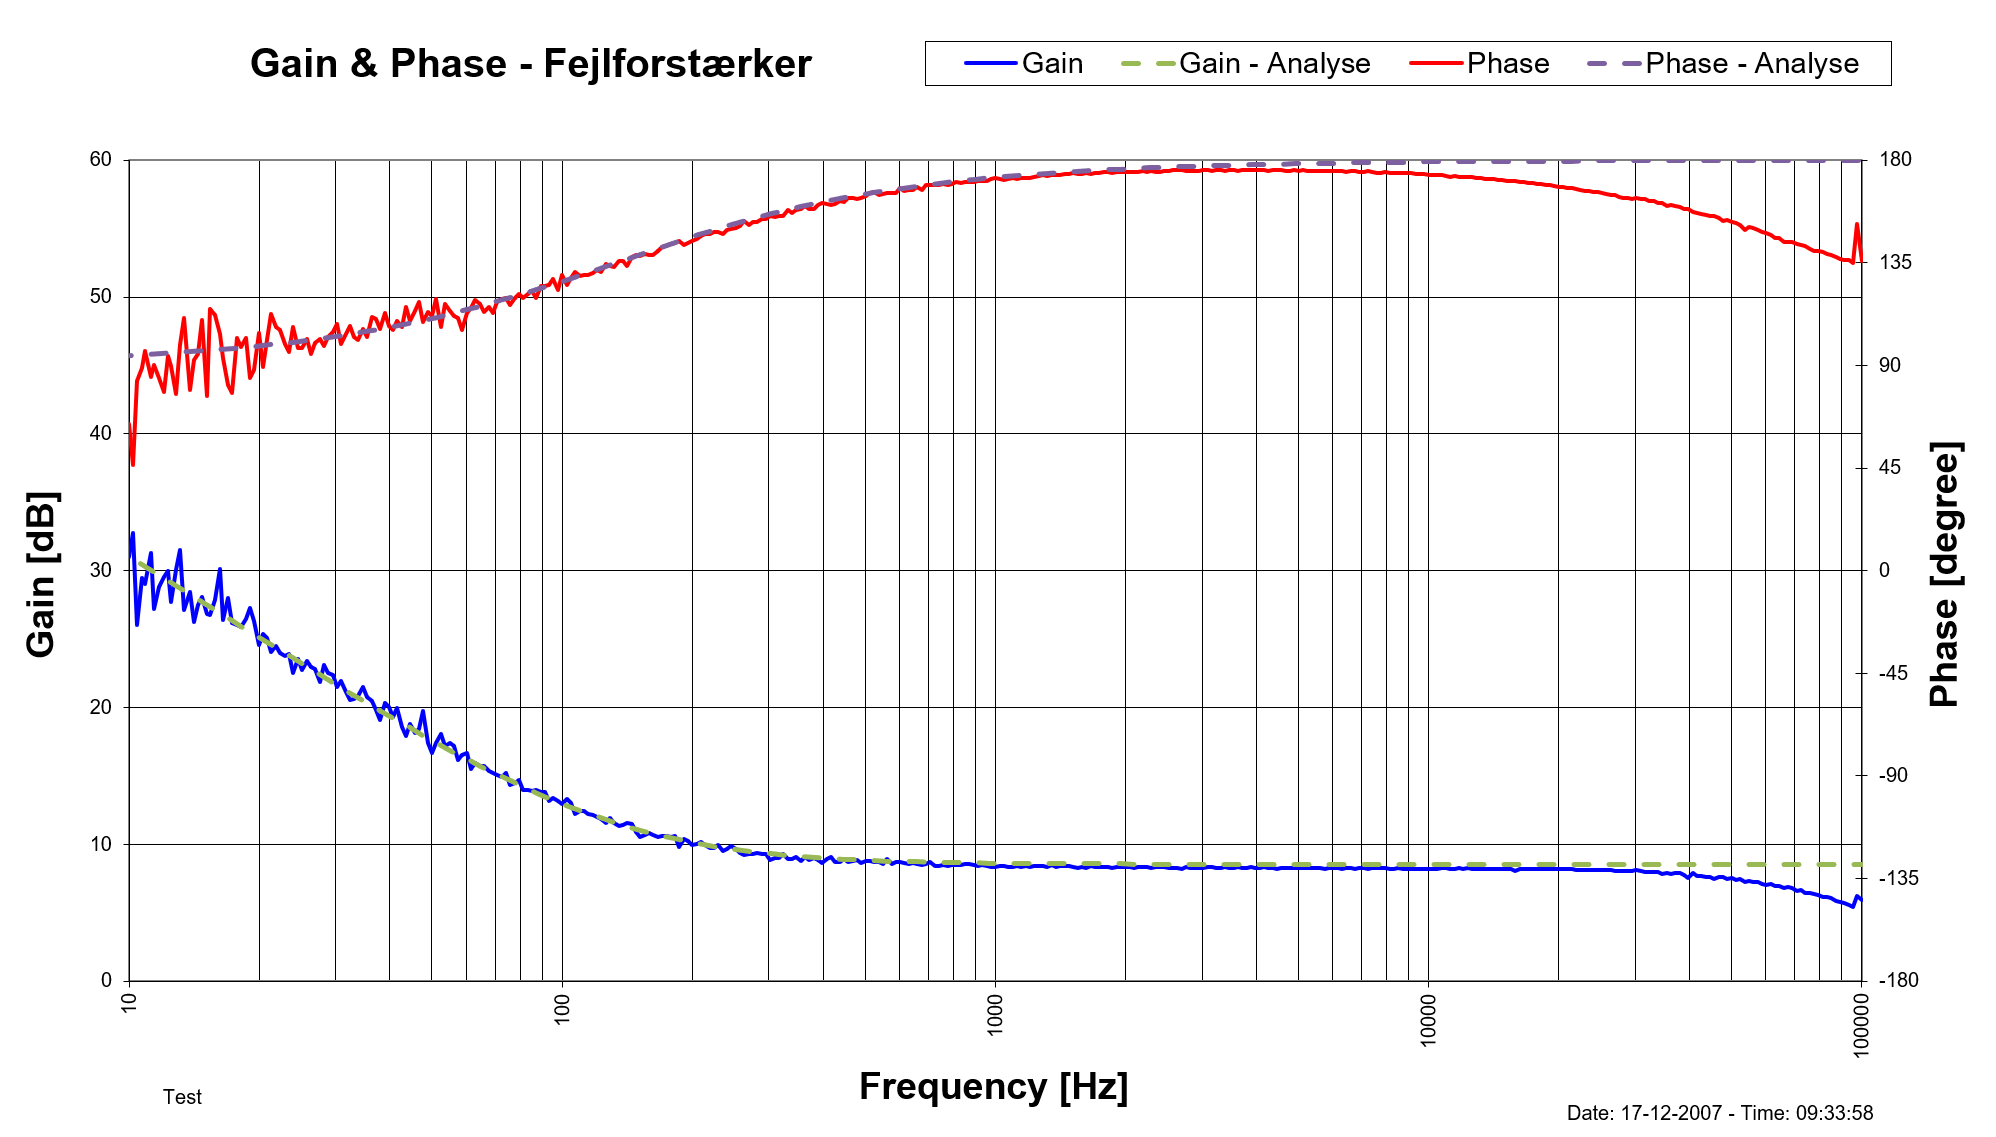
\includegraphics[max width=0.7\linewidth]{/tex/3iteration/billeder/Realisering/Realisering_gain_fase_opamp.PNG}
	\caption{Realisering af fejlforstærkeren}
	\label{fig:Realisering_error_op_amp_3}
\end{figure}

\noindent Bode plottet for det samlede system er vist på figur~\ref{fig:Realisering_total_3}. Her måles der over den modstand, hvor fejlsignalet indføres. Det svarer til at måle fra indgangen af fejlforstærkeren til udgangen af converteren. Gain for realiseringen er den blå, mens gain for analysen er den grønne stiplede. Fasen for realiseringen er den røde, mens fasen for analysen er den stiplede lilla. På bode plottet ses det, at der er en større afvigelse ved højere frekvenser. Det kan se ud til, at der er en pol i systemet, der ikke er taget højde for i analysen. Da dette sker ved frekvenser hvor gain-margin skal aflæses, bliver denne måling usikker. Den aflæses dog til $14.5\decibel$, hvilket er en afvigelse på $4.5\decibel$ ift. analysen. Fasemargin og båndbredden aflæses til henholdsvis $69.8^\circ$ og $3.86k\hertz$, hvilket stemmer med det forventede. 

\begin{figure}[H]
	\center
	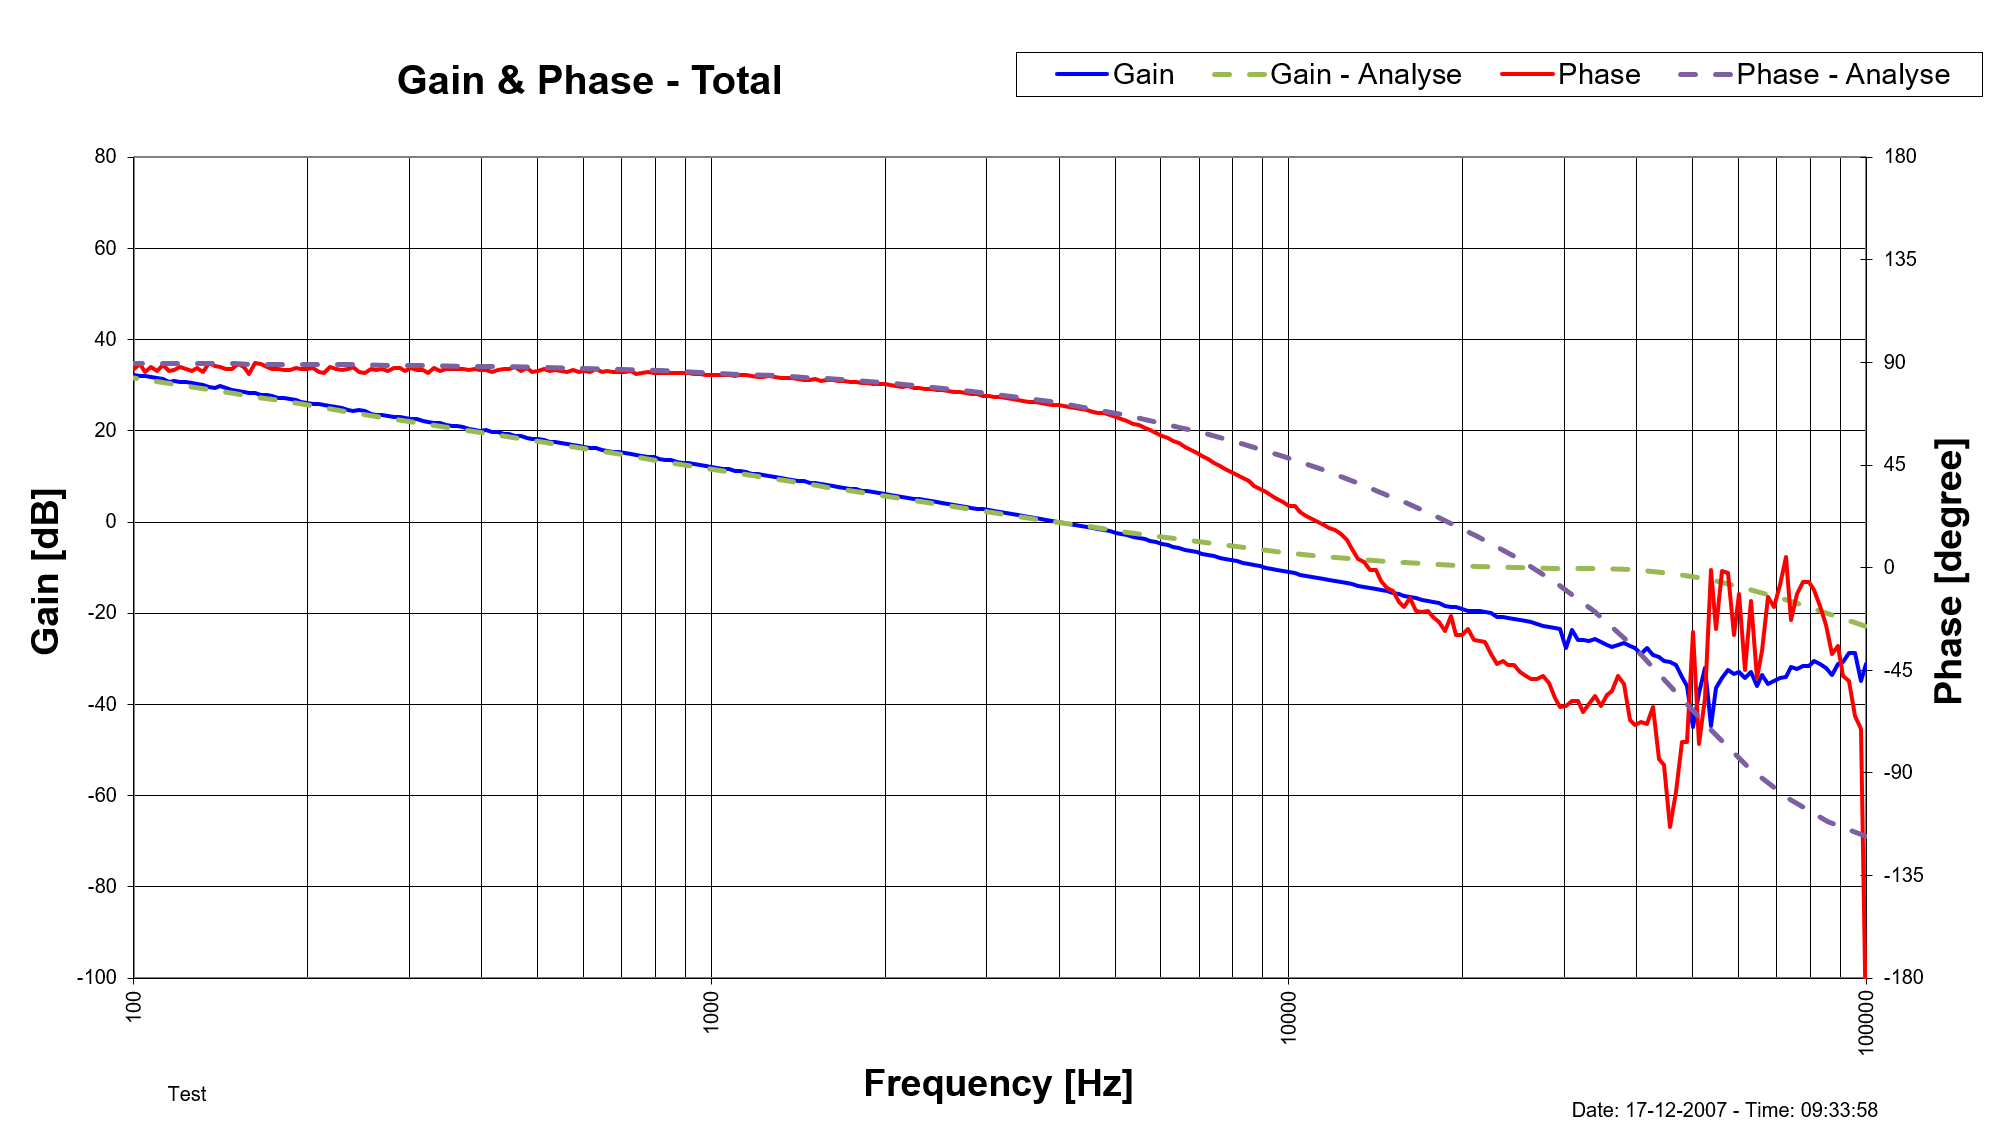
\includegraphics[max width=0.7\linewidth]{/tex/3iteration/billeder/Realisering/Realisering_gain_fase_total.PNG}
	\caption{Gain-fase måling af det samlede system}
	\label{fig:Realisering_total_3}
\end{figure}

\noindent Bode plottet for det samlede system måles også med maksimal inputspænding på 50V. Dette er vist på figur~\ref{fig:Realisering_total_50V_3}. Her er forstærkningen blå, og fasen er rød. Gain-margin aflæses til $14.3\decibel$, fasemargin aflæses til $76.3^\circ$, og båndbredden aflæses til $5.7k\hertz$. Dette viser, at systemet er stabilt ved både lav og høj inputspænding.

\begin{figure}[H]
	\center
	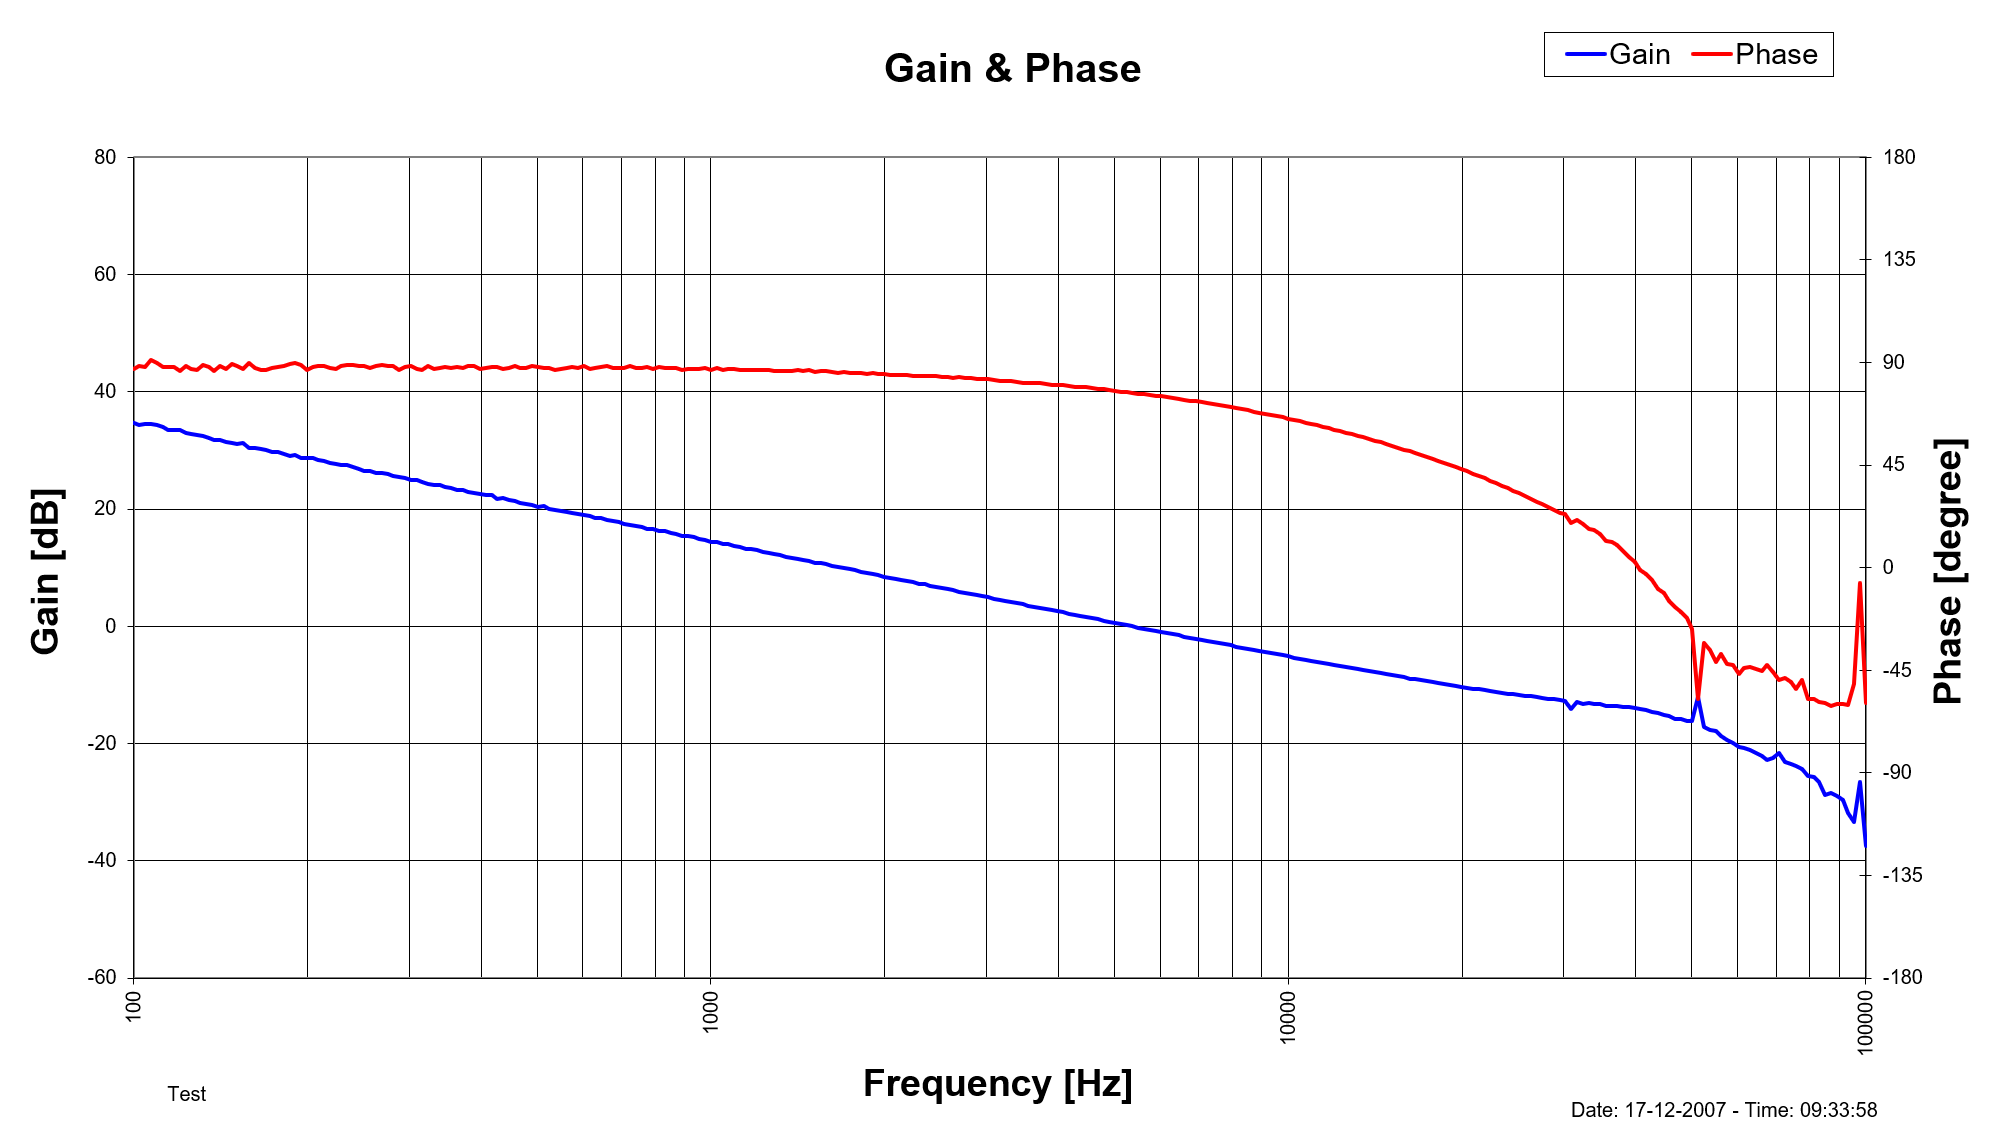
\includegraphics[max width=0.7\linewidth]{/tex/3iteration/billeder/Realisering/Realisering_gain_fase_total_50V.PNG}
	\caption{Gain-fase måling af det samlede system - 50V inputspænding}
	\label{fig:Realisering_total_50V_3}
\end{figure}







\subsection{Load step}
Igen er load steppet realiseret som det blev gjort i load step sektionen ~\ref{loadsteprea} under 2. iteration. Resultatet af dette ses på ~\ref{fig:loadstep3}
\begin{figure}[H]
	\center
	\includegraphics[max width=0.7\linewidth]{/tex/3iteration/billeder/realisering/Loadstep.PNG}
	\caption{Realiseret load step}
	\label{fig:Loadstep3}
\end{figure} 
Det er tydeligt at overshootet er faldet en del med den forstørrede båndbredde. På ~\ref{fig:loadsteprise} er der zoomet ind på dykket, der hvor loaden skifter til at være $10\ohm$.
\begin{figure}[H]
	\center
	\includegraphics[max width=0.7\linewidth]{/tex/3iteration/billeder/realisering/Loadsteprise.PNG}
	\caption{Zoom på dyk ved $10\ohm$}
	\label{fig:Loadsteprise}
\end{figure}
Dette dyk aflæses til at være ca. $300mV$, hvilket skal ses i forhold til de $700mV$ fra tidligere. Til gengæld er reguleringstiden steget med omkring $0.5mw$ til $2ms$. På ~\ref{fig:loadstepfall} ses istedet stigningen, da der igen kobles $20\ohm$ på som load.
\begin{figure}[H]
	\center
	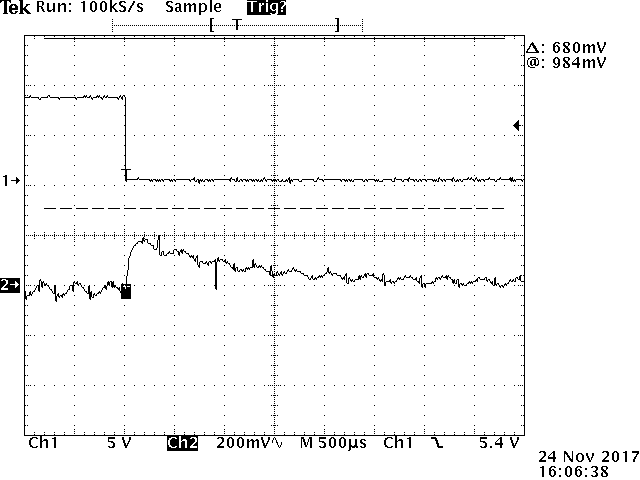
\includegraphics[max width=0.7\linewidth]{/tex/3iteration/billeder/realisering/Loadstepfall.PNG}
	\caption{Zoom på stigning ved $20\ohm$}
	\label{fig:Loadstepfall}
\end{figure}
Her aflæses stigningen til $200mV$ i forhold til de tidligere $600mV$ og igen er reguleringstiden steget med ca. $0.5mw$ til $2ms$. 

%%%% Realisering af tab efter optimerng %%%%

\subsection{Tab}

\subsubsection{MOSFET}
Det nye tab i MOSFET'en bestemmes ved, at måle temperaturstigningen i af kølepladen, og ud fra den termiske modstand, beregne tabet. 

\subsubsection{samlet tab}



\clearpage

% Konklusion

\chapter{Konklusion}
Målet med projektet var, at udvikle en DC/DC converter, som skal kunne indgå i et universelt aktiveringskredsløb. Her skulle det være muligt, at tilpasse converteren til to forskellige belastningstyper. 

Der er blevet implementeret en funktionsdygtig converter, med en statisk udgang. Desuden opfylder converteren de fleste krav for den valgte udgangsbelastning. Samtidig er der blevet lagt et grundlag, og gjort nogle overvejelser, for videreudviklingen af converterens udgangstrin. 

Der er udviklet en converter med hurtig og stabil regulering. Reguleringen overholder kravene til gain- og fasemargin for den valgte belastning, inden for hele indgangsspændings-intervallet. Desuden overholder den præcisionskravene for både udgangsstrøm og -spænding, ved den valgte belastning. 

Der er blevet gjort overvejelser ift. et optimalt termisk design. Der er løbende i projektet blevet optimeret på dette punkt, men det endelige resultat er ikke tilfredsstillende. Desuden vil dette tab blive større hvis udgangsbelastningen øges. Derfor er der blevet gjort nogle overvejelser for, hvordan kravet vil blive overholdt. 

Der er opstillet en funktionel P-spice model, der giver et præcist indblik i converterens funktionalitet. Modellen er så tilfredsstillende, at stort set samtlige funktionaliteter kan eftervises. Der er dog mindre afvigelser, da modellen for den ønskede MOSFET ikke kunne skaffes.

